 \documentclass[11pt, a4paper,twoside]{tesi_upf}
%CODIFICATION
\usepackage[utf8]{inputenc}
%LENGUAGE
\usepackage[english]{babel}
%ONLY TO OBTAIN MARK BANK INDEX INDICATION B5
\usepackage[a4paper]{geometry}
\usepackage[cam,a4,center,frame]{crop}
\usepackage{epigraph}
\usepackage{listings}
\usepackage{xurl}
\usepackage{subfig}
\usepackage{float}
\usepackage{enumitem}
\setlist[itemize]{noitemsep, topsep=0pt}
\setlist[enumerate]{noitemsep, topsep=0pt}
\setcounter{secnumdepth}{3}

%INCLUDE GRAPHICS AND THE LOGO OF THE UPF
\usepackage{graphicx}
%FONTS TIMES OR GARAMOND, 
\usepackage{times}
%\usepackage{garamond}

%WITHOUT HEADINGS: NO MODIFICATION
\pagestyle{plain}
%FOR THE INDEX OF SUBJECTS
\usepackage{makeidx}
\makeindex
%BIBLIOGRAPHY STYLE
\bibliographystyle{vancouver.bst}
%SELECT LANGUAGE
\selectlanguage{english}

%THE TABLE OF CONTENTS IS TITLE CONTENTS
%\addto\captionscatalan
%  {\renewcommand{\contentsname}{\Lar%ge \sffamily Sumari}}


%ADD YOUR DATA
\title{Malware and Spy Systems}
\subtitle{P2P Botnets over Tor}
\author{Daniel Orihuela Rodríguez}
\thyear{2019-2020}
\department{ICT (Information and Communications Technology)}
\supervisor{Xavier Salleras Soler}


\begin{document}
\frontmatter
\maketitle
\cleardoublepage

\setlength{\parskip}{1em}
\renewcommand{\baselinestretch}{1.50}\normalsize

\emph{"I don't want to live in a world where everything that I say, everything I do, everyone I talk to, every expression of creativity, or love, or friendship is recorded, and that's not something I'm willing to support, it's not something I'm willing to build, and it's not something I'm willing to live under"}

\rightline{---Edward Snowden, 2013.}
\clearpage


%%%%%% Thanks
\noindent {\Large \sffamily Acknowledgements}

I cannot thank enough all the people that directly or indirectly helped me making me doing that project. My family for always helping me with my studies, to keep going. My coworkers, for the flexibility and the knowledge that indirectly help me with my project. Xavier Salleras, for supervising my project, helping me with all the doubts that I had, and knowing how to guide me. For the ideas, and the freedom to do whatever I wanted and push me to improve them. Without him, this project would have looked so much different.

\cleardoublepage
%%%%%% End of thanks

%ABSTRACT IN TWO LEGUAGES.
\selectlanguage{english}
\section*{\Large \sffamily Abstract}

In the last decade, cybercrime has been a profitable area. Cybercriminals had been able to get away with large amounts of money thanks to advanced techniques and architectures like botnets, ransomware, banking malware, rootkits, and many more; that is giving them the possibility to make huge profits with a high level of security and anonymity.

In this project, we will see how cybercriminals design, program, and deploy botnets. Which are their intentions, and how will this impact in the implementation. How a botnet can be used as a spy system to steal user information, and we will develop one to show its potential. In our case, it will be a P2P botnet that will hide in Linux machines with the help of a rootkit and will communicate through Tor. This will help us understand the motivation of a cybercriminal, their tools, and how can we protect ourselves against them.

\selectlanguage{english}
\vspace*{\fill}
\section*{\Large \sffamily  Resumen}

En la última decada, el cibercrimen ha sido una área muy lucrativa. Cibercriminales han sido sido capaces de llevar a cabo actividades ilegales, generando un gran vólumen de beneficios financieros para ellos mismos gracias a técnicas avanzadas y arquitecturas utilizadas como botnets, ransomware, programas maliciosos enfocados a bancos, rootkits y muchos más. Gracias a estas herramientas, son capaces de ganar una gran cantidad de dinero con un alto grado de anonimidad y seguridad.

En este proyecto veremos como los cibercriminales diseñan, programan y desplegan botnets. Aprenderemos cuales son las intenciones de estos individuos o grupos. Como puede variar el diseño de estos sistemas, dependiendo el enfoque que le quieran dar. Como pueden utilizarse las botnets para espiar a los usuarios y robarles información confidencial. Diseñarmos e implementaremos una botnet con un protocolo P2P y utilizará herramientas, como los rootkits, para operar en el sistema a favor del atacante sin ser detectado. Las comunicaciones irán a través de Tor. Todo esto nos ayudará a entender las motivaciones de los cibercriminales, sus herramientas y como podemos protegernos.

\vspace*{\fill}

\cleardoublepage
%END OF ABSTRACT

%PREFACE. 
{\bf Preface}
%\section*{\Large \sffamily  Preface}

I have always liked computers. Small machines that connect people in different parts of the world and transform electrical signals into video and audio, among other things. I wanted to learn how all this works, and how it is possible. Even now, in my last year of Computer Engineering, many things seem magical, although I can understand the gears spinning behind them.

I started programming before I enrolled in Computer Engineering and it is something I have always liked. Building programs to make people's lives easier is one of my main interests.  However, there is one topic that cannot be left out due to it's ubiquity to any area of the computer world, cybersecurity. This was not an important topic until recently. Cybercrime is on the rise and it is increasingly common for user data to be leaked due to vulnerability flaws.

For these reasons, I decided to learn everything I could about cybersecurity. To be able to apply this knowledge to the applications and systems I will be involved in the future, and protect the users. Apart from the fact that it's a really fun topic.

\cleardoublepage
%END OF PREFACE

\setlength{\parskip}{0em}
\renewcommand{\baselinestretch}{1}\normalsize
%TABLE OF CONTENTS: REQUIRED
\tableofcontents

\setlength{\parskip}{1em}
\renewcommand{\baselinestretch}{1.50}\normalsize

%lIST OF FIGURES; ONLY IF THERE ARE FIGURES
\listoffigures
%TO APPER THE LIST OF FIGURES IN THE TABLE OF CONTENTS 
\addcontentsline{toc}{chapter}{List of figures}

%LIST OF TABLES; ONLY IF THERE ARE TABLES
\listoftables
%TO APPEAR THE LIST OF TABLES IN THE TABLE OF CONTENTS
\addcontentsline{toc}{chapter}{List of tables}

%START THE TEXT
\mainmatter
\chapter{Introduction}

Cybersecurity and privacy are fields in continuous expansion, especially since the unveiling of various massive global surveillance projects from the NSA (National Security Agency) by the hand of Edward Snowden \footnote{More information can be found in Citizenfour documentary or his Permanent Record book} in 2013. Julian Assange preceded Edward Snowden with his page called "WikiLeaks" which could be found leaked information from the United States Army in 2010. This has not stopped and in 2018 Cambridge Analytical suffered a big scandal when it was discovered that they have been harvesting people's personal information without consent from their Facebook profiles, and used this information for political advertising purposes, tipping the balance.

This project aims to study how an espionage system works. How this system reaches our networks and computers, how are we infected and how can they steal our data. For this, we are going to program Malware, which is nothing more than a program designed specifically to perform malicious actions. With this, we will build a botnet, which is a group of internet-connected devices controlled by the master to carry out bad-natured actions.

\section{Motivation}

We like a lot of different topics inside the computer-engineering world, but we consider cybersecurity one of the most interesting, fun, and stimulating ones. Trying to break different applications or protocols can make you learn a lot more than just doing them, and at the same time, you are helping to improve the security of these projects. Ideally, preventing cyber criminals from discovering and exploiting them.

Lately, awareness around privacy concerns had increased since the discovery of projects to gather sensitive information or companies that misused this data, like the ones presented in the introduction. For this reason, this project is going to consist of learning how this system works, we will create one of myself and we will try to point the weak points and how to evade being in one of those espionage systems.

With this information, we hope that anybody that reads this dissertation can understand how these systems work, how are they deployed and which security measure could be applied to stop them. In the best of cases, without user interaction.

\section{Main Problem}

The problem we want to solve can be summarized in one question: How do we design a system that allows us to obtain information from different victims without their knowledge in such a way that it is very difficult to reach us and potentially disclosing our identity?

People able to answer this question could be using their knowledge for bad purposes like cybercriminals. They could be also using it for legit purposes, fighting terrorism, like the NSA. The main concern here is the misuse of these tools to invade people's privacy.

Even though botnet is a word mostly related to mischievous, there are legitimates uses for botnets. Distributed systems are botnets used to solve a problem among a large number of nodes (machines connected to the system that work towards a common goal). Amazon Web Services, for example, owns a huge botnet with which they can offer services to companies and developers.

So Botnets do not just allow to obtain information from nodes. If done properly you can also make them work for you, this can go from Distributed Denial Of Service (DDoS) attacks to the training of Deep Learning Neural Networks.

\section{Proposed Solution}

Creating a botnet implementing protocols to avoid leaking IP addresses or any kind of personal information is hard and time-consuming. 

What we propose is to use any kind of already working network that gives this anonymity to us, like Tor \footnote{More information in \url{https://www.torproject.org/}} or I2P \footnote{More information in \url{https://geti2p.net/en/}} for the communication between the victims connected to our botnet. This way we can focus our efforts on adding functionalities: execution of commands, updating of the code, establishing tunnels to use victims as anonymizers (machines that forward messages so that the origin is hidden from the recipient), etc. For this dissertation, we will be using Tor since it is a very well-known anonymous network.

Our botnet will consist of a set of victims infected with malicious software to send private information to the master assuring its anonymity through Tor.


\chapter{Technical Background}

Espionage systems are supported above different tools, concepts, and techniques that make them work as expected and without risking themselves. We will discuss and talk deeply about them and some more targeted knowledge we need to acquire before moving on with the Proof of Concept.

\section{Malware}

There are numerous types of malware-free on the Internet and in the different systems connected to it. Virus, worms, trojans, backdoors, adware, ransomware, ... .However, some of these are more interesting than others when it comes to spying users. We will focus on these especially, besides the malware that helps us staying and hiding in the system.

\subsection{Worm}

This piece of software is capable of spreading copies of itself from computer to computer over a network. It is very dangerous since no human interaction or program is required. This type of malware has been the most serious security threat since 1988 \cite{worm} and was used as the first digital weapon (i.e., Stuxnet \cite{stuxnet-book}).

The main task of worms is to spread over the network taking advantage of software vulnerabilities. They can even carry a payload that enables them to modify or delete files from the system. However, they are extremely difficult to control since they tend to provoke side effects (e.g., an increase in the consumed bandwidth over the network).

\subsection{Spyware}

One of the oldest types of malware, specifically designed to gather sensitive information about individuals like: visited websites, usernames, passwords, downloaded files, and many more; used to earn money either by selling it on the black market or blackmailing the concerned person.

After being infected with spyware, you could end being the victim of identity theft or credit card fraud. Both being extremely annoying situations. Notice in figure \ref{fig:fraud_figure} how more than 50\% of user complaints fall under the identity theft or fraud categories over the years.

\begin{figure}
    \centering
    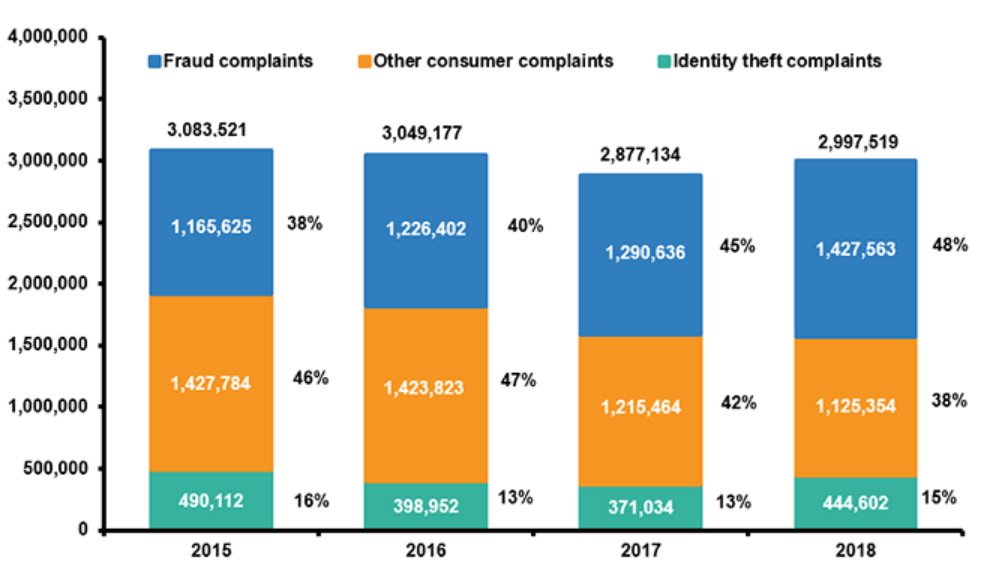
\includegraphics[width=\linewidth]{images/fraud_victims.png}
    \caption{Quantity of frauds and percentages by type in the United States. Reprinted from iii.org 
    \cite{fraud_graph}.}
    \label{fig:fraud_figure}
\end{figure}

\subsection{Fileless Malware}

Fileless Malware, Non-malware, Memory base, or living-off-the land are different names for a type of malware which rather than using malicious software, uses legitimate tools already installed in the system to execute commands. Since an executable is not being used because they live in the RAM, they barely leave any trace. Therefore, these are extremely useful for avoiding detection by traditional antivirus. Another advantage is that you cannot simply blacklist the software since it is probably being used by the employees (e.g., PowerShell).

Example: We are navigating the internet and we enter into a website that requires Adobe Flash Player. It turns out that the version of the Adobe Flash Player installed in our system is vulnerable and allows us to run commands in the browser memory. As you can see, commands are stored and executed from memory. By no means, a file is downloaded to execute the malicious code.

\subsection{Trojan}

This is the master of deception among all types of malware. This malware does what the user thinks it does, but in addition to that, it is performing malicious actions in the background without the user knowledge.
\interfootnotelinepenalty=10000
A Trojan is no more than a facade that gives the user a feeling of trustiness. Is like a legitimate software with malicious software inside. Cybercriminal seems to be using this technique especially with android games that target kids, expecting that young child install them on one of their parent's phones
\footnote{News about android games \url{https://www.forbes.com/sites/zakdoffman/2020/03/24/google-confirms-malicious-kids-games-hiding-on-play-store-delete-these-66-apps-now/}}.

No wonder it is named after the famous strategy performed in the myth of the Trojan War.

\subsection{Backdoor}

A mean used for accessing systems bypassing the required authentication methods. It is used for legitimate purposes like restoring passwords or being able to troubleshoot remotely. But surely, people will know it better for its mischievous uses.

Cybercriminals may want to gain persistent access to a system once it has been infected. Notice that with the previously mentioned types of malware we cannot access or control the machine once it has been infected, it will just execute a predefined set of commands. That is precise, what backdoors allow us to do. However, it will leave a trace in the system (e.g., open port, running process, a new user in the database) and they will be exposed to the user, if not previously considered.
 
\subsection{Rootkit}

Union of Root (user with privileges in a Unix-like operating system) and kit(set of software compounds implemented in the tool), is a type of malware used for hiding the malware once it found a host.

A rootkit is one of the most powerful types of malware out there. There is only one requirement for this to work, we must have root permission in the infected machine so that we can successfully hide any potential trace from the user/admin of the system. Given that we have root permissions in the system, we can do anything we want: mess with the memory, change system files, modify them, overwriting the memory with zeros, etc. For that reason detecting rootkits is hard, once you are infected, they have the power to change the outputs given but any program in your machine (antivirus included).
\newpage
Operating Systems have a mechanism to protect data called Protection Rings (See figure \ref{fig:protection_ring_figure}). It is a set of rings which different privileges. This concept is important since there exists different types of rootkits, the main ones being: user-mode rootkit, kernel-mode rootkit, and bootkit, and each one operates at a different level.

\begin{figure}
    \centering
    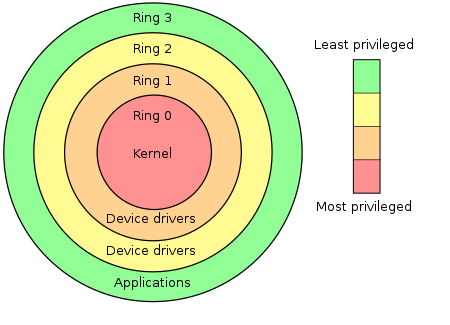
\includegraphics[scale=0.35]{images/protection_ring.png}
    \caption{Protection ring. Reprinted from cs.rutgers.edu 
    \cite{protection_ring_graph}.}
    \label{fig:protection_ring_figure}
\end{figure}

\subsubsection{User Mode Rootkit}

User-mode rootkits operate on the third ring, along with the rest of the applications. They can hide files and change system behaviour, the drawback is that kernel code can detect this kind of rootkits. Moreover, they are easier to remove since the user only needs to remove the piece of software from the system.

Usually, the attack vector of user-mode rootkits come the Operating System libraries (e.g., .dll file in Windows).


\subsubsection{Kernel Mode Rootkit}

Kernel-mode rootkit operates on ring zero. They live in the kernel (i.e., the core computer program of an Operating System allowing the communication between hardware and software), so they have the most privileges and can do whatever they want without the user's knowledge. This time, the kernel code will not be able to detect a kernel rootkit. Since they operate on the same level, the rootkit can modify kernel code at will. Furthermore, to remove such a rootkit the user will need to reinstall the Operating System.

\subsubsection{Bootkit}

Boot level rootkits work as replacements for bootloaders. Do the same as previous rootkits but it is harder to remove. The user will need to reinstall the bootloader, which is not an easy task.

\section{GNU/Linux}

Contrary to people believe, Linux is not the Operating System but the kernel itself \footnote{Linux and the GNU System \url{https://www.gnu.org/gnu/Linux-and-gnu.html}}. GNU is an Operating System that accepts various kernels, even though it is commonly paired with the Linux kernel.

\subsection{Distributions}

There are hundreds of different distributions that uses Linux as its kernel. Ubuntu, Debian, Fedora, Arch Linux, Trisquel, Kali Linux, etc. 

Each distribution is a packet containing some software on top of a modified Linux Kernel. That little detail that each distribution makes some changes to the Linux Kernel may seem like nothing, but it is important to take into account if you are trying to develop malware that targets the Linux Kernel on different distributions.

Beware is that on the internet you can find different machines with the same flavour of Linux (e.g., Ubuntu) but different Linux Kernel versions (i.e., one machine can have Linux Kernel 4.18.17 while another has version 2.6.26), the same way it can happen with Windows and their different versions. However, the number of possible combinations is wider.

\subsection{Virtual File System}

In Linux, everything is a file or considered as such. This is a simplification of the reality that helps understand how the kernel works.

Virtual File System (VFS) is an abstraction of a File System that works as an interface between the kernel and the File System in use. So, it does not matter if you are using EXT4 or EXT3 that the system calls done for performing files operations will remain the same, as long as the implementation for the specific File System is correct (i.e., the functions open(), read() and write() need to be implemented).
From a Software Engineering point of view, this is awesome. It allows us to have a cleaner code that does the same calls regardless of the implementation. Furthermore, that is the reason why it is said that in the Linux Kernel everything is a file. Some information is stored in VFS and they behave like a file (e.g., hardware or process information), even though they are not. To demonstrate that is enough to check the size of files in different parts of the system. For example, /proc, which is a VFS in Linux that stores process and system information, and as you can see in \ref{fig:all_is_a_file}, directories size are 0, that demonstrates that these are not real files. They are temporarily stored in the Kernel's internal cache.

\begin{figure}
    \centering
    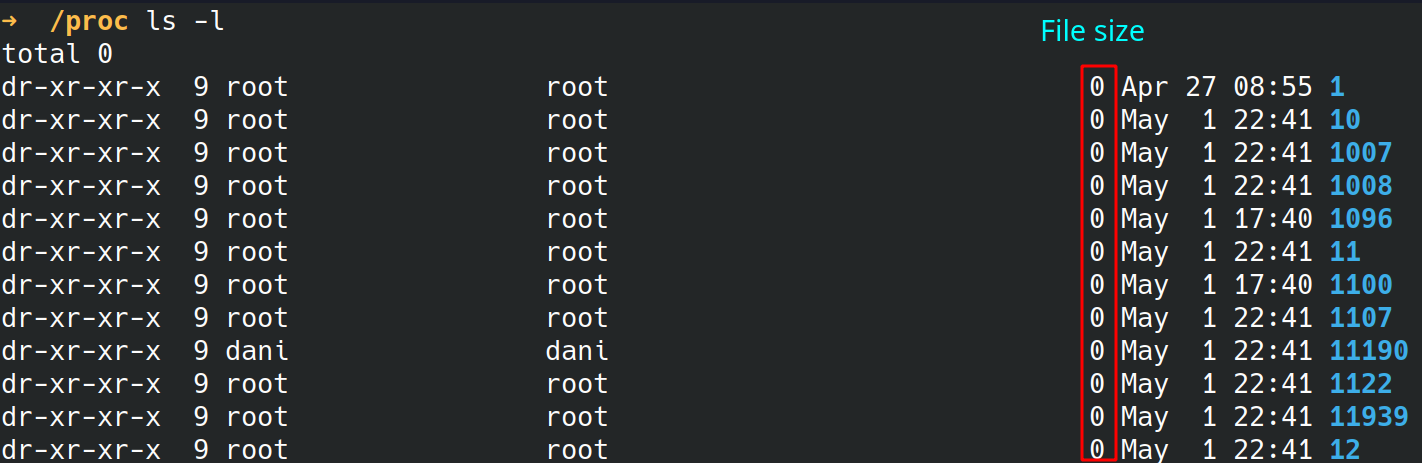
\includegraphics[width=\linewidth]{images/all_is_a_file.png}
    \caption{/proc directory content}
    \label{fig:all_is_a_file}
\end{figure}

We can find several VFS in the Linux Kernel: /proc, /etc, /sys, /tmp, /dev, /dev/null, etc. As you can see, the use of VFS is not isolated, it is used extensively in the kernel. Each of these storing different information that we will take into account when preparing our malware.

\subsection{Linux Kernel}
The Linux Kernel is a free and open-source (FOSS) Unix-like Operating System Kernel. It is the most well known Unix-like we are aware of. At the time of writing this the GitHub (Service for projects that use a version control called Git) repository has over 900.000 commits and 300 Pull Requests (improvements from other programmers waiting to be reviewed by a contributor of the project to be accepted or rejected).

The Linux Kernel is monolithic, which means that the entire Operating System is working on the kernel space (Ring 0 in \ref{fig:protection_ring_figure}) and is alone in the supervisor mode (i.e., just the Operating System is trusted code and can access memory and hardware directly). All other software is run in the user mode since it is considered untrusted. For this reason, code cannot mess with the kernel code. However, we can interact with resources thanks to an Application Programming Interface (API) which contains functions called "system calls" (the only entry point to the kernel).

Getting a GNU/Linux distribution into doing something in the kernel space for our profit can be tricky, but we will learn how in section \ref{solution}.

\subsection{Loadable Kernel Modules}
\label{loadable-kernel-module}

A Loadable Kernel Module (LKM) is a file or set of files that can extend the kernel code to add new system calls, add drivers for some devices, or modify the current behaviour of the system.

The main goal is to be able to easily load and unload these modules to the kernel without the need to have it written in the Operative System (OS) kernel. So anyone, without the need of being working in Microsoft for example, can extend the OS kernel. Another advantage is that you do not need to reboot the computer to reload the code, it will immediately available.

Despite being an excellent solution, it can carry security concerns. If you have your machine compromised, the attacker could take advantage of an LKM to stay hidden in the system by modifying the normal behaviour of system calls, making it harder for other programs to detect the infection.

\section{Anonymity Network (Tor)}
\label{tor-section}

The Onion Router, best known as Tor after the acronym, is a free open source project whose ambition is to enable people to use the internet anonymously (i.e., enabling people to connect to a server in a way such that anyone looking at the connection cannot know the origin nor the actual recipient). One legit use case is using Tor for accessing censored services in some countries.

\subsection{Tor Virtual Circuits}

Virtual Circuits allow the communication between two machines as if they were connected with a dedicated physical link, even though if they are not. In Tor, virtual circuits are created to allow the flow of data between two machines (origin and recipient) securely (i.e., encrypted tunnel).

In figure \ref{fig:virtual_circuit} we can see the connection created between Alice and Bob. Communications are secured through symmetric keys exchanged with the Diffie-Hellman key exchange method.

\begin{figure}
    \centering
    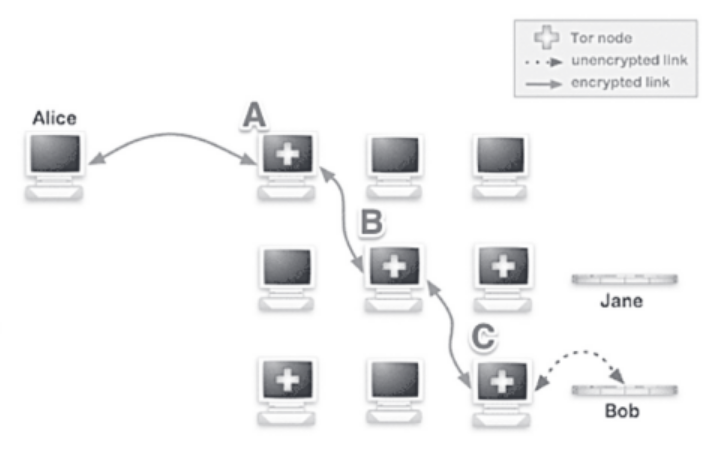
\includegraphics[scale=0.5]{images/virtual_circuit.png}
    \caption{Tor communication protocol, origin to recipient
    \cite{botnet-over-tor}.}
    \label{fig:virtual_circuit}
\end{figure}

The Diffie-Hellman method is as follows:
\begin{enumerate}
    \item Alice and Bob decide some common parameters: modulus $p$ and base $g$.
    \item Alice chooses a secret integer $a$ and sends $A=g^a mod p$ to Bob.
    \item Bob chooses a secret integer $b$ and sends $B=g^b mod p$ to Alice.
    \item Alice obtains the secret key $s=B^a mod p$
    \item Bob obtains the secret key $s=A^b mod p$
    \item Both Alice and Bob have a common secret key.
\end{enumerate}
\newpage
Given the steps above for negotiating keys between Alice and Bob, we can easily build a virtual circuit:
\begin{enumerate}
    \item Alice negotiates a symmetric key with computer B, using Computer A as an anonymizer.
    \item Alice negotiates a symmetric key with computer C, using Computer A and B as anonymizers.
    \item At this point, we have a virtual circuit as the one in figure \ref{fig:virtual_circuit} and Alice can communicate with Bob anonymously.
\end{enumerate}

It is important to notice that all the traffic is encrypted from hop to hop, except from computer C to Bob, where the data is being sent in plain text. That is because each computer of the circuit removes one encryption layer from the message. In the beginning, the message has three encryption layers. Computer A removes the first layer, computer B removes the second layer and computer C removes the last layer. Therefore, computer C obtains the plain text that can be sent to the destination.

What we described above in a sequence of steps can be seen in the following figure.

\begin{figure}[h]
    \centering
    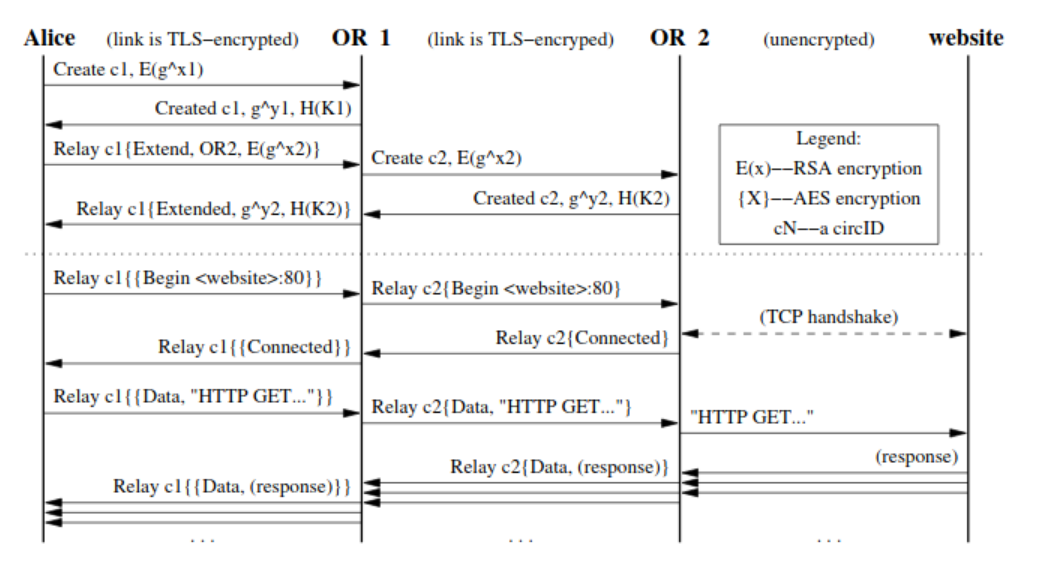
\includegraphics[scale=0.4]{images/build_two_hops_circuit.png}
    \caption{Two hop circuit creation followed by the fetch of a webpage information
    \cite{tor-whitepaper}.}
    \label{fig:two_hop_circuit}
\end{figure}

\subsubsection{Guards}

Tor virtual circuits are made of three machines, that connect the origin with the recipient machine. Each machine is a guard, and there exist three types of guards.

\begin{itemize}
\item\textbf{Entry guard:} First machine in the circuit. This machine knows the origin.

\item\textbf{Relay:} Second machine in the circuit. Forwards encrypted messages from entry to exit nodes. Knows nothing about the message, the origin, and the recipient.

\item\textbf{Exit relay:} Last machine in the circuit. It knows the message, since traffic is not encrypted, and the recipient.
\end{itemize}

\subsubsection{Path Length}
\label{path-length}

Tor virtual circuits are always made of three nodes, and it is not without reason. Nevertheless, it was a problematic issue that was extensively debated.

Using one guard no more will not give any benefit to the end-user, is like using any other ordinary anonymizer. The anonymizer will know the origin, the message, and the recipient.
A circuit made of two guards is a better approach, even though it is not good enough. In the event an adversary owns the exit node, they would immediately know which the entry guard is, and therefore which machine to compromise to get to the origin. A three-guard scheme fixes this problem because, even if the adversary owns the entry or exit node, he will not be able to get the other end (there is a node in the middle). Furthermore, owning the middle machine (i.e., relay) does not help the adversary because the message is encrypted both when receiving from the entry guard and when sending it to the exit node  \footnote{Why does Tor use only 3 relays: \url{https://www.quora.com/Why-does-Tor-use-only-3-relays}} \cite{master-tor-circuit}.

Nevertheless, no system is 100\% secure. If the adversary has control over the entry and the exit nodes, he would be able to link the recipient with the IP address of the origin given enough data.

A common mistake is to think that following the above reasoning, adding more nodes would increase security.
It is not very clear the effects of that. Adding more nodes will make it harder for a compromised entry or exit node to reach the other end. Furthermore, no middle relay will know both, entry and exit relays, and will also require to compromise all the middle relays to reach both ends. Besides, the probability of taking a compromised node for the circuit is higher, even though it remains the same for picking a compromised entry or exit node. However, if by chance we end on a circuit with the entry and exit nodes, the adversary only needs enough traffic data to correlate \cite{master-tor-circuit}.

Three seems the perfect path length for enough security with a decent speed connection.

\subsubsection{Types of Circuits and Rotation}

Different types of circuits exist for different use cases. Furthermore, Tor tries to predict which type of circuit will be needed shortly to build it.

A circuit can be internal or external. It is internal if the user is visiting an Onion Service (i.e., anonymous webpage, we will talk further in section \ref{onion-service-section}). Otherwise, if the user is trying to access a server outside the Tor network it falls under the external category. Moreover, they can be fast and/or stable. Fast circuits are made of nodes with enough bandwidth while stable requires of nodes with sufficient uptime (i.e., the time a machine has been up and running). Tor prefers fast circuits for internal and external traffic, while it prefers stable circuits for services like FTP or SSH that require long-lived connections.

At startup, Tor creates a fast exit circuit and two fast internal circuits. From that moment on, it will try to predict if more circuits are needed and from which type.

User does not always use the same circuit since it will increase the risk of leaking its IP address. Every ten minutes the circuit is changed, therefore reducing the time a node on the path can observe the traffic \footnote{For more info on guards \url{https://blog.torproject.org/improving-tors-anonymity-changing-guard-parameters}}.

\subsection{Onion Services} \label{onion-service-section}

Onion services, also known as hidden services, are Internet services (i.e., webpages, servers, admin panels, ... that a user can access through the Internet) with the added plus of anonymity granted by Tor in this case. These services are exposed over the Tor network and cannot be accessed from the outside \cite{onion-services-tor}.

Onion services directions are strange and difficult to remember (e.g., $vww6ybal4bd7szmgk\\cyruucpgfkqahzddi37ktcso3ah7ngmcopnpyyd.onion$). The direction is the hash of the onion service public key. Where a hash is an output obtained from a Hash function that receives something as input and returns an alphanumerical string of a fixed size. Furthermore, these services cannot be found with a search engine (i.e., Google, Bing, Yahoo, etc), since they are not indexed by search engines (i.e., an onion service cannot appear as one of the results returned by a search engine). Is the owner of the onion who decides to make the direction public (e.g., on a blog, webpage, or any other social network).
In \cite{onion-services-tor}, the researches did some surveys to find out how people discover onion services. The three most popular ways are social networks like Twitter or Reddit, special search engines for onion services such as Ahmia \footnote{Ahmia search engine \url{https://ahmia.fi/}} and randomly while browsing the web, given that the owner published the direction. Another way could be onion domain aggregators like the Hidden Wiki. It is a normal webpage accessible from the Internet where you can find a list of onion services along with their names.

Onion services are servers that offer anonymity since the user does not know the server and the server does not know the user. However, we did not see yet which is the mechanism that enables this.

\subsection{Rendezvous Points}

Rendezvous points are nodes in the Tor network that allow communication between users and hidden services without leaking IP addresses of users and servers.

Rendezvous points are more important than they may seem at first. Besides hiding the server and user IP from each other, they disable potential Denial Of Service (DoS) attacks since the IP of the server is unknown. Nonetheless, introduction points are open and you could attempt to DoS them to disable access to the onion service. However, the service can re-advertise itself at different introduction points; the attacker can decide to share the introduction points with only the people he wants, restrict the volume of requests or even require a certain amount of computation for every request.

The protocol works as follows \cite{tor-whitepaper}:

\begin{enumerate}
    \item Server creates a public key for the hidden service.
    \item Server selects at random some nodes to work as introduction points, which are published to the lookup service (i.e., directory servers, we will talk about them in the next section).
    \item Builds virtual circuits to each introduction point. \item Introduction points wait for user's requests to the hidden service.
    \item User types the onion service in the search bar. In the background:
    \begin{enumerate}
        \item Retrieve onion information from the lookup service.
        \item Select a node at random to use as a rendezvous point.
        \item User builds a circuit to the rendezvous point.
        \item User sends a message to a random introduction point of the onion service.
        \item Server receives the message and if the server accepts the message, it will build a circuit to the user rendezvous point.
    \end{enumerate}
    \item The user and the server established a connection.
\end{enumerate}

\subsection{Directory Authorities}

Directory Authorities or Directory Servers are special well known and trusted nodes of the Tor network. Without them, Tor would be so slow.

Directory Authorities store information about the network state along with the list of routers. This way, users can now at every moment the state of onions and the network. Onion routers send information periodically to these onions services, which combine this information with their information on the network. The joined information constitutes what is called a "directory" of the entire network state \cite{tor-whitepaper}.

Client Tor software comes with a list of directory authorities stored to have an initial view of the network. Furthermore, directory authorities have a special mechanism to automatically approve new nodes. They do not advertise by default unrecognized onion routers, otherwise, an adversary could take advantage. An adversary could even control a directory authority. Therefore, directory authorities are synchronized and they must agree on a common directory and the client should only trust the directory returned by this consensus \cite{tor-whitepaper}.

\subsection{Attacks}
\label{tor-attacks}

Tor design makes a lot of sense and they have taken into account a lot of factors. However, it is impossible to make a 100\% secure system and Tor is no exception. In this section, we will talk about some attacks that could seriously damage user anonymity and therefore, cybercriminals using Tor for their botnet communication protocol.

\subsubsection{Sybil Attack}

An attack in which a node in a peer to peer network behaves like multiple identities instead of only one. It is directly affected by the difficulty to create identities, how the system accepts identities without any type of link to a trusted identity, and whether the system treats all entities equally.
Notice, that you can have a machine that has multiple identities or you can be in control of multiple machines with one identity each.

An example of a Sybil attack is the 51\% attack that can affect blockchain networks. Blockchain networks have a consensus protocol to reach the truth (e.g. if a transaction is valid or not in Bitcoin). If an adversary manages to get control of 51\% of the nodes, the truth is whatever the adversary says is the truth.

This kind of attack is cheap to perform if the network does not have any type of explicit or implicit Certification Authority \cite{sybil-attack} like is the case of the Tor network. Tor has already been attacked with such a strategy in 2014 by Lizard Squad \footnote{Sybil attack to Tor \url{https://www.theregister.co.uk/2014/12/27/tor_lizard_squad_sybil_attack/}}. Nevertheless, Tor has put in place some monitoring software in case they fall under attack again.

\subsubsection{Deanonymize Hidden Service Client}

Users accessing a specific hidden service can be deanynomized, therefore leaking their IP address.

Tor code is publicly available, so in theory, anyone can:

\begin{enumerate}
    \item Download the code.
    \item Modify the code.
    \item Introduce a modified node to the Tor network.
\end{enumerate}

For instance, some researches have developed an attack where they modified the messages that are sent and received by the hidden service and a relay. Therefore, if for some reason a client is connected to the modified hidden service using a modified entry node, they can locate the client comparing the logs in the entry node and the hidden service \cite{deanonymize-clients-hidden-service}.

As with the next attack, it is very unlikely to happen. But given an adversary with enough resources, it could be done.

\subsubsection{Traffic Correlation}

One way of deanonymizing users is by correlation with their traffic.

This is probably the most well-known attack that a user could suffer in the Tor network. The technique consists of introducing or comprising as many nodes as possible in the Tor network, therefore increasing the probability that a user picks an entry and exit node from the adversaries set. This will allows the adversary to analyze the traffic and get complete or partial information about the user. \cite{tor-correlation-master, tor-whitepaper}. Remind that it does not matter the path length, the adversary just needs entry and exit node as mentioned in section \ref{path-length}. E.g., An adversary introduces a delay in the information channel and try to highlight a specific virtual circuit of all the virtual circuits he has. If the circuit is formed by entry and exit nodes in his power, he can get all the info. User IP address from the entry node, the message, and server IP address from the exit node.

Despite these techniques being possible to perform, Tor has a lot of people volunteering with nodes so it should not happen as it is impractical to obtain a huge enough quantity of nodes.

These are not the only attacks that can be done, there are three main categories: directory attacks, active attacks, and passive attacks, as described in the tor white paper \cite{tor-whitepaper}. However, we believe the most important are the ones mentioned above, these are the ones that will shape our botnet design.

\section{Botnet}
\label{section:botnets}

A botnet is a group of machines connected to the internet controlled that usually works towards the same goal (e.g., sending spam emails, mining bitcoins, train a machine learning model). A botnet is strongly associated with criminal actions, but there are also legit botnets (e.g., Amazon Web Services, clusters, SETI@home project to analyze radio signals in search of extraterrestrial intelligence \footnote{SETI@home official page \url{https://setiathome.ssl.berkeley.edu/}}. Botnets are powerful systems, but we must know the different topologies we can give to them since they will give different advantages and disadvantages.


\subsection{Command and Control}

The simplest botnet follows a centralized topology. All nodes are connected to a central machine, called the Command and Control (C\&C) server. It is a dedicated machine for communicating with the different nodes.

All nodes are connected to the central server, which results in low latency and high scalability. The disadvantage is that it has a single point of failure, the central server. If someone attacks the server, the botnet stops working. The master could add more C\&C servers. This would be more resilient, but still subject to the same kind of attacks (e.g. DoS). The resiliency could be further improved with Domain Generation Algorithms (DGA) to generate the C\&C domains \cite{botnets}. This way the botnet would be able to generate the domain where the victim should connect (e.g. DGA that generates new domains based on the current date). The attacker can register the domains when needed since he knows the DGA implementation. Nonetheless, DGA implementations can be reverse-engineered. Therefore, susceptible again to the same kind of attacks.

A good example of a C\&C server is Mirai. This botnet is famous because it managed to pull off some serious DDoS attacks, the most powerful reaching 1 Tbit/s of data. The heaviest DDoS attack we are aware of.

\subsection{Peer to Peer}

Peer to peer (P2P) topologies does not have any type of central server. Every node in the botnet is at the same level and can perform server and client actions.

This structure increases the resiliency since every node can behave like the C\&C server, but we removed the single point of failure.
The bad side is that depending on how we make the connection between nodes, we will have other difficulties. For example, if we decide that any given node is connected to every node, it will be robust and will not matter that a node is removed but it is not going to be scalable. However, we can make it not fully connected, which will help us with the scalability but reduce robustness and make the implementation harder. In the end, it will depend on the number of nodes we may need to connect to the botnet.

Other points must be taken into consideration, like setting up the botnet. With a P2P is not easy, we could for example hard code a set of initial peers in the bot executable. So every new node knows who to talk with. The problem here is that this group of initial peers become the single point of failure. This could be improved making the new node randomly scan the internet for peers \cite{botnets}.

Finally, a P2P protocol must be used for the communication between nodes that are not directly connected (i.e., nodes need to be able to forward messages).

Botnets examples could be DUSTBot or Zeus.

\subsection{Hybrid}

Both C\&C and P2P topologies present weaknesses. The hybrid approach exists to try and take the best parts of the previously mentioned structures.

We need three layers to create a hybrid botnet. A layer for nodes, a layer for proxies (nodes that forward messages), and a layer for the C\&C servers. Then, it is just a matter of adding some nodes as proxies and some bots to make the work \cite{botnets}. Other approaches exist depending on which part of the botnet could be improved with P2P and which parts could be improved with centralization.

Some examples are Miner, Storm, or Sality version 3 \cite{botnets}.

\begin{figure}
    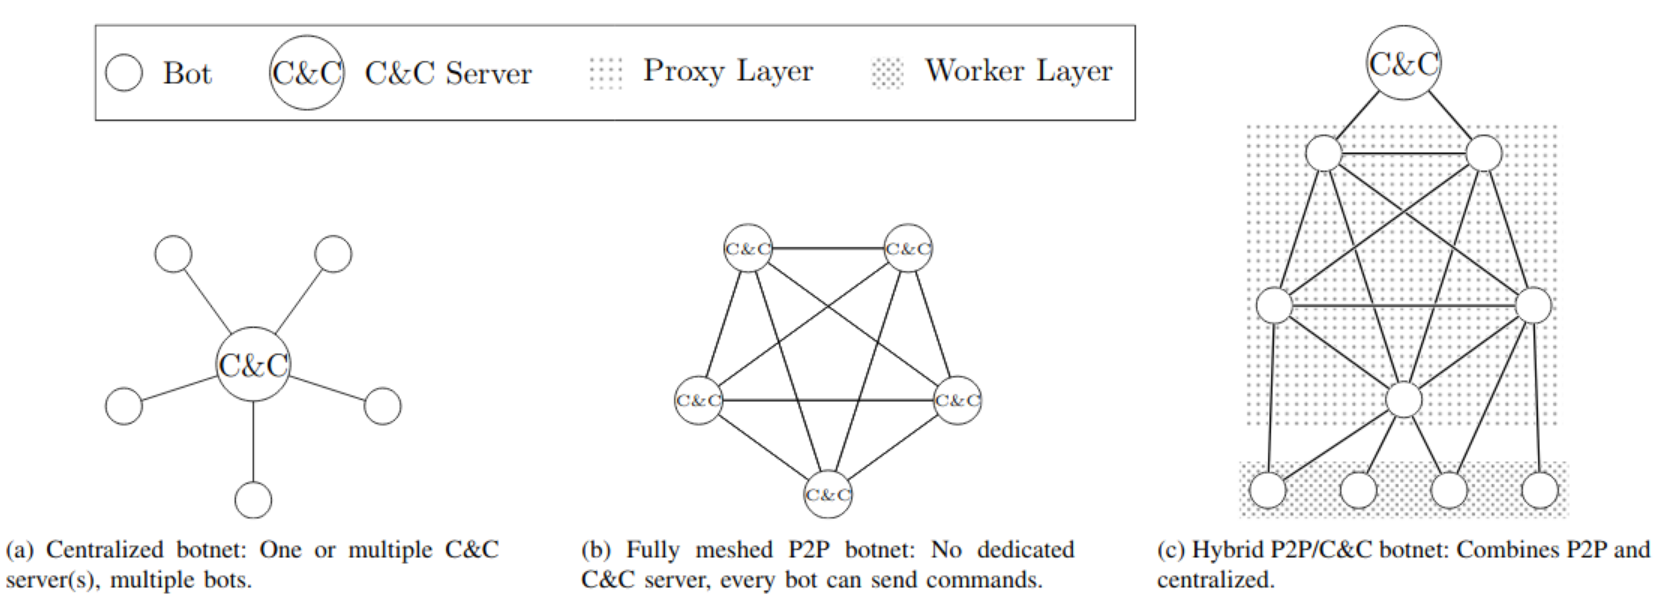
\includegraphics[width=\linewidth]{images/botnets.png}
    \caption{Botnets topologies
    \cite{botnets}}
    \label{fig:botnets-topologies}
\end{figure}

\begin{table}
    \resizebox{\textwidth}{!} {
        \begin{tabular}{||c | c | c||}
            \hline
            Botnet Type & Advantages & Disadvantages \\ [0.5ex] 
            \hline\hline
            Command and Control & Easy set up & Single Point of Failure
            \\
            & Low Latency & \\
            & High Scalability & \\
            \hline
            Peer to Peer & No Single Point of Failure & Difficult to set up \\
            &  Variable Latency & Needs forwarding commands support\\
            & & Handle node removal\\
            \hline
            Hybrid & Flexibility & Needs thorough thought\\
            & & Difficult design\\
            & & Difficult implementation\\
            \hline
        \end{tabular}
    }
    \caption{Botnets topologies comparison}
\end{table}

\chapter{Tools}

We want to mention the tools required for the implementation of the botnet, what do they do, and why are we using them.

\section{C Programming Language}

C is an imperative programming language that provides low-level access to memory. It is difficult to master but its low-level nature helps when you need to control hardware for example. The Linux kernel is written in C and Assembly Language, therefore we will use C for programming our rootkit to hide the malware in the victim machine.

\section{Python Programming Language}

Python is a multi-paradigm programming language. It is specially used by people inside the data science and machine learning world due to the huge quantity of libraries with incredibly useful tools for these areas. However, it has a lot more (e.g., cryptography libraries). We decided to use python for the ease of use and availability of different libraries with cryptographic tools.

\section{Virtual Machines}

Virtual Machines are computer system emulations that can be executed inside another computer. This will let us emulate different computers to test the correct functioning of the botnet. Various tools exist to emulate computers, we decided to use Virtual Box since we were already familiar with it. Using another program should not make any difference.

We thought about using docker. However, it makes use of the host operating system and this would give us a problem when testing the rootkit.

\section{Tor}

Tor is a network that helps with anonymous communication. We have already talked extensively in section \ref{tor-section}. We will use it to make the victims' communication between each other and with the master more secure.

\section{Loadable Kernel Modules}

Loadable Kernel module is a program that gets introduced into the kernel to extend its functionality. We have already discussed this topic too, in section \ref{loadable-kernel-module}. It will help us get infiltrated into the Linux kernel and hide our malware.

\chapter{State of the Art}

We have good knowledge of the basic theory and the tools and how they work behind. However, this is not enough, we must know about the new malware trends, which backdoors are preferred by cybercriminals and the reason, which botnets have been deployed in the last years and what computer scientist researchers have discovered, among others.

\section{Exploits and Backdoors} \label{section:exploits-and-backdoor}

Exploit is a piece of code that takes advantage of bugs or vulnerabilities present in the system to cause unanticipated behaviour. Backdoor is a technique to gain access that allows us to bypass normal authentication methods. We need both of them to infect a machine, an exploit to gain access to the system, and a backdoor to keep coming back (for a limited or undefined period).

The difficult part is identifying the infection vector (i.e., the method used to infect a machine and spread the malware). Making a backdoor is the easy part, we just need something that gives us access (e.g., a new user in the system). 

Changing files or binaries of the system is how backdoors are made. Probably, the easiest backdoor would be to manually add a user. E.g., you are with a friend and he needs to go to the toilet, then you are left with his computer wide open. You could decide to create a new user account without his knowledge, and you would have created a backdoor to his system. Even though an easier one to spot. 
A seasoned hacker would probably change some binaries. E.g., Linux kernel uses PAM (Pluggable Authentication Modules), these modules allow us to configure how authentication and other security measures behave \footnote{More about PAM in \url{https://www.linux.com/news/understanding-pam/}}. In figure \ref{fig:original-pam} we can see a fragment of pam\_unix\_auth.c \footnote{Source code \url{https://github.com/linux-pam/linux-pam/blob/master/modules/pam_unix/pam_unix_auth.c}}(file in charge of authenticating a user), in which it is being verified the given password for the given user (i.e., if the password is correct).

\begin{figure}
    \centering
    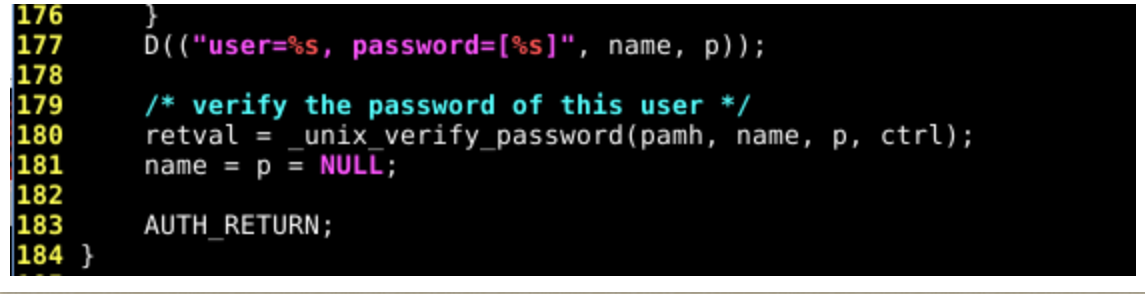
\includegraphics[width=\linewidth]{images/original_pam.png}
    \caption{Original pam\_unix\_auth.c file. Reprinted from Le journal d'un reverser
    \cite{pam-tutorial}.}
    \label{fig:original-pam}
\end{figure}

To introduce a backdoor we just need to check if a specific password is given; otherwise, we let the program run as it would normally do. Check figure \ref{fig:backdoor-pam}. As you can see, we introduced a backdoor in just two lines of code. The difficult part is to infect a machine without the user noticing.

\begin{figure}
    \centering
    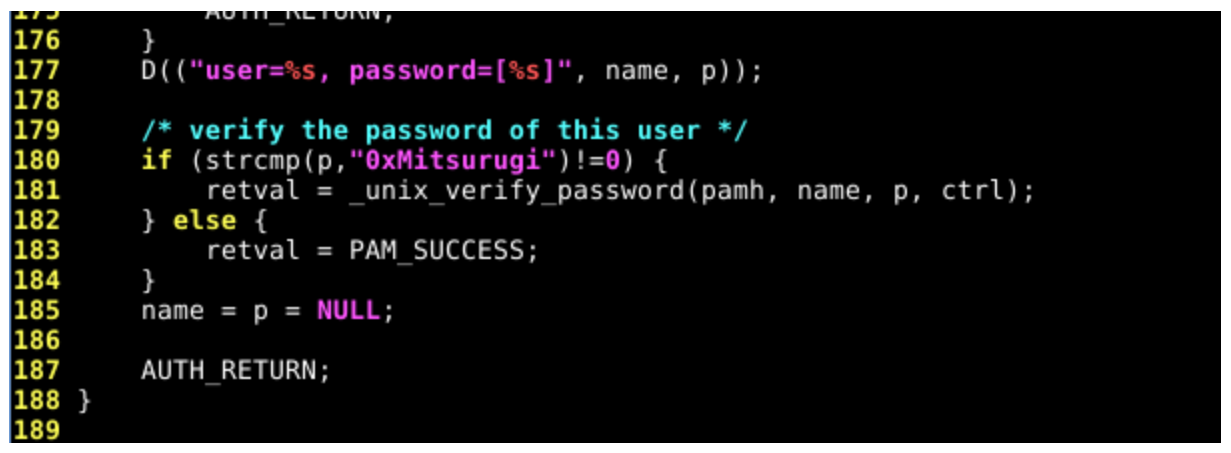
\includegraphics[width=\linewidth]{images/pam_backdoor.png}
    \caption{pam\_unix\_auth.c file with backdoor. Reprinted from Le journal d'un reverser \cite{pam-tutorial}.}
    \label{fig:backdoor-pam}
\end{figure}

Just to give another example, there is a technique called "Magic ICMP" \footnote{An implementation of this can be seen in \url{https://github.com/f0rb1dd3n/Reptile}}. Assume already have an infected machine under control. If that is the case, we could insert a piece of code to execute an action on the event that a crafted packet is sent to the port where we are listening. This way, an attacker could send a specially designed packet to spawn a reverse shell on his computer, for example. A reverse shell is a technique in which the attacker machine will behave as the server and the victim will connect to it, giving remote access to the attacker.

As we demonstrated backdoors are easy. The difficult part is finding and infection vector so that every machine you reach is infected without user knowledge. Usually, attackers use vulnerabilities that can be found either in the OS or an application that allows arbitrary execution of code, privilege escalation, or both. Arbitrary execution of code allows executing code in a machine without the user knowledge, while privilege escalation allows executing code with an unprivileged user as if it were the administrator. These are some infection vectors, but they cannot match the impact that social engineering has. Social engineering is the art of fooling people to perform actions or disclosing private information to you. Usually, you need user interaction to install the malware into the system. Otherwise, it is just really complicated. Nowadays, computers always ask the user for permission to perform any kind of action: download files, download files from unknown origins, open files, execute programs, watch videos... Therefore, manipulating the user to download and open a file, for example, becomes crucial for the success of your malware. If you are targeting a person you need to trick him. If you are targeting a whole network, you only need to trick the admin or trick a user and try to exploit vulnerabilities to move laterally or escalate privileges. Social engineering is most of the time the first step for a hack.

The biggest threat regarding malware is probably zero-days. Unknown vulnerabilities by the people who want to stop them.
Every day new vulnerabilities are found. A zero-day exploit consisting of an SQL injection (i.e., executing a command by sending a specially crafted message to the SQL database) issue was found on Sophos XG Firewall that may have allowed remote code execution \footnote{More on the vulnerability \url{https://nvd.nist.gov/vuln/detail/CVE-2020-12271}}. Cybercriminals tried to use this exploit to plant backdoors and various types of malware on different companies \footnote{More on the attack and response: \url{https://www.bankinfosecurity.com/hackers-tried-to-exploit-zero-day-flaw-in-sophos-firewall-a-14325}}.

A security researcher from the Eindhoven University found a vulnerability in Thunderbolt connections that could allow hackers to get all the information on the laptop in 5 minutes, just using some components costing a few hundred dollars \cite{thunderbolt}.

One of the most important commands in Linux is sudo, it allows users to execute programs as an administrator. Therefore, this command must have no flaws in its code. However, it had some flaws in the past, and a new one was discovered at the time we were writing this. This vulnerability allows us to execute commands as root, even though the user does not have root permissions \footnote{Sudo vulnerability CVE: \url{https://access.redhat.com/security/cve/cve-2019-14287}}.

Microsoft had a serious vulnerability in his Teams workplace video chat and collaboration platform. The problem is how they handle authentication to image resources. When the app is opened an access token is created, which allows users to see shared images. An attacker was able to obtain a cookie called "authtoken" that grants access to a resource server. With this, they could perform some actions like sending messages. Furthermore, two of the subdomains were susceptible to takeovers. Therefore, if the attacker gets a user to visit a subdomain which he has previously taken over, he could get a new "authtoken" that grants him the power to access the Team data \footnote{New explaining Microsoft flaw \url{https://thehackernews.com/2020/04/microsoft-teams-vulnerability.html}}.

Exploits are our best allies (from an attacker's point of view), they will help us get into any system we want. Otherwise, we have our hands tied. Backdoors are just the next step after exploitation.

\section{Botnets}

Botnets, from a cybercriminal point of view, is a group of infected machines that an attacker uses for its benefit. Some use cases are: sending spam emails, selling the computational power to third people, stealing personal and sensitive information. They have and are being used widely, either for making money (the cybercriminals use case) or for fighting against terrorism (the intelligence agencies). Although it violates people's rights to privacy.

In 2016 a malware research group found out the existence of a botnet, following a Command and Control architecture. It would become famous due to the successful launch of the most destructive DDoS attack done in the whole history. Moreover, no other botnet has surpassed the amount of data reached (1 Tbit/s) by that botnet, which is known as Mirai. The attack appears on the "Notable Recent Attacks" section of a webpage that paints on a map the top daily DDoS attacks, see figure \ref{fig:digital-attack-map-notable-attacks}. We can see the attack in figure \ref{fig:mirai-ddos}. That botnet had such a huge impact that a lot of new botnets based on Mirai started to come out. Even nowadays, new variants keep appearing. Mukashi, a variant of Mirai, appeared shortly after the appearance of a Proof of Concept (PoC) illustrating how to exploit a new vulnerability affecting Zyxel NAS devices in March of 2020 \cite{palo-alto}. \textbf{Side note:} Proof of Concepts are good for sharing knowledge, and should not be a problem because they are always made public after the vulnerability has been patched. Nonetheless, there will always be unpatched devices. Ideally, all devices should be patched as fast as possible or cybercriminals will try and get the advantage of that. You should update your devices as fast as possible.

\begin{figure}
    \centering
    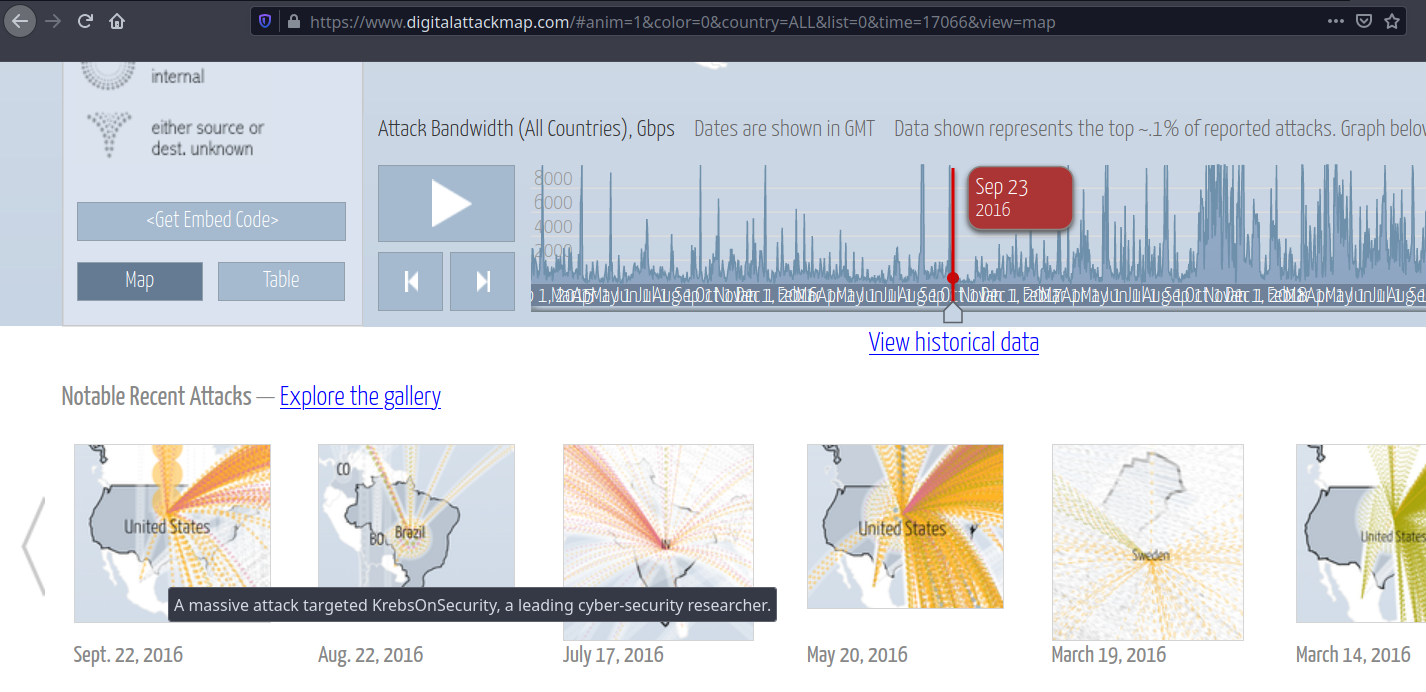
\includegraphics[width=\linewidth]{images/ddosmap-index.png}
    \caption{Mirai DDoS appears in Notable Recent Attacks sections inside Digital Attack Map webpage}
    \label{fig:digital-attack-map-notable-attacks}
\end{figure}

\begin{figure}
    \centering
    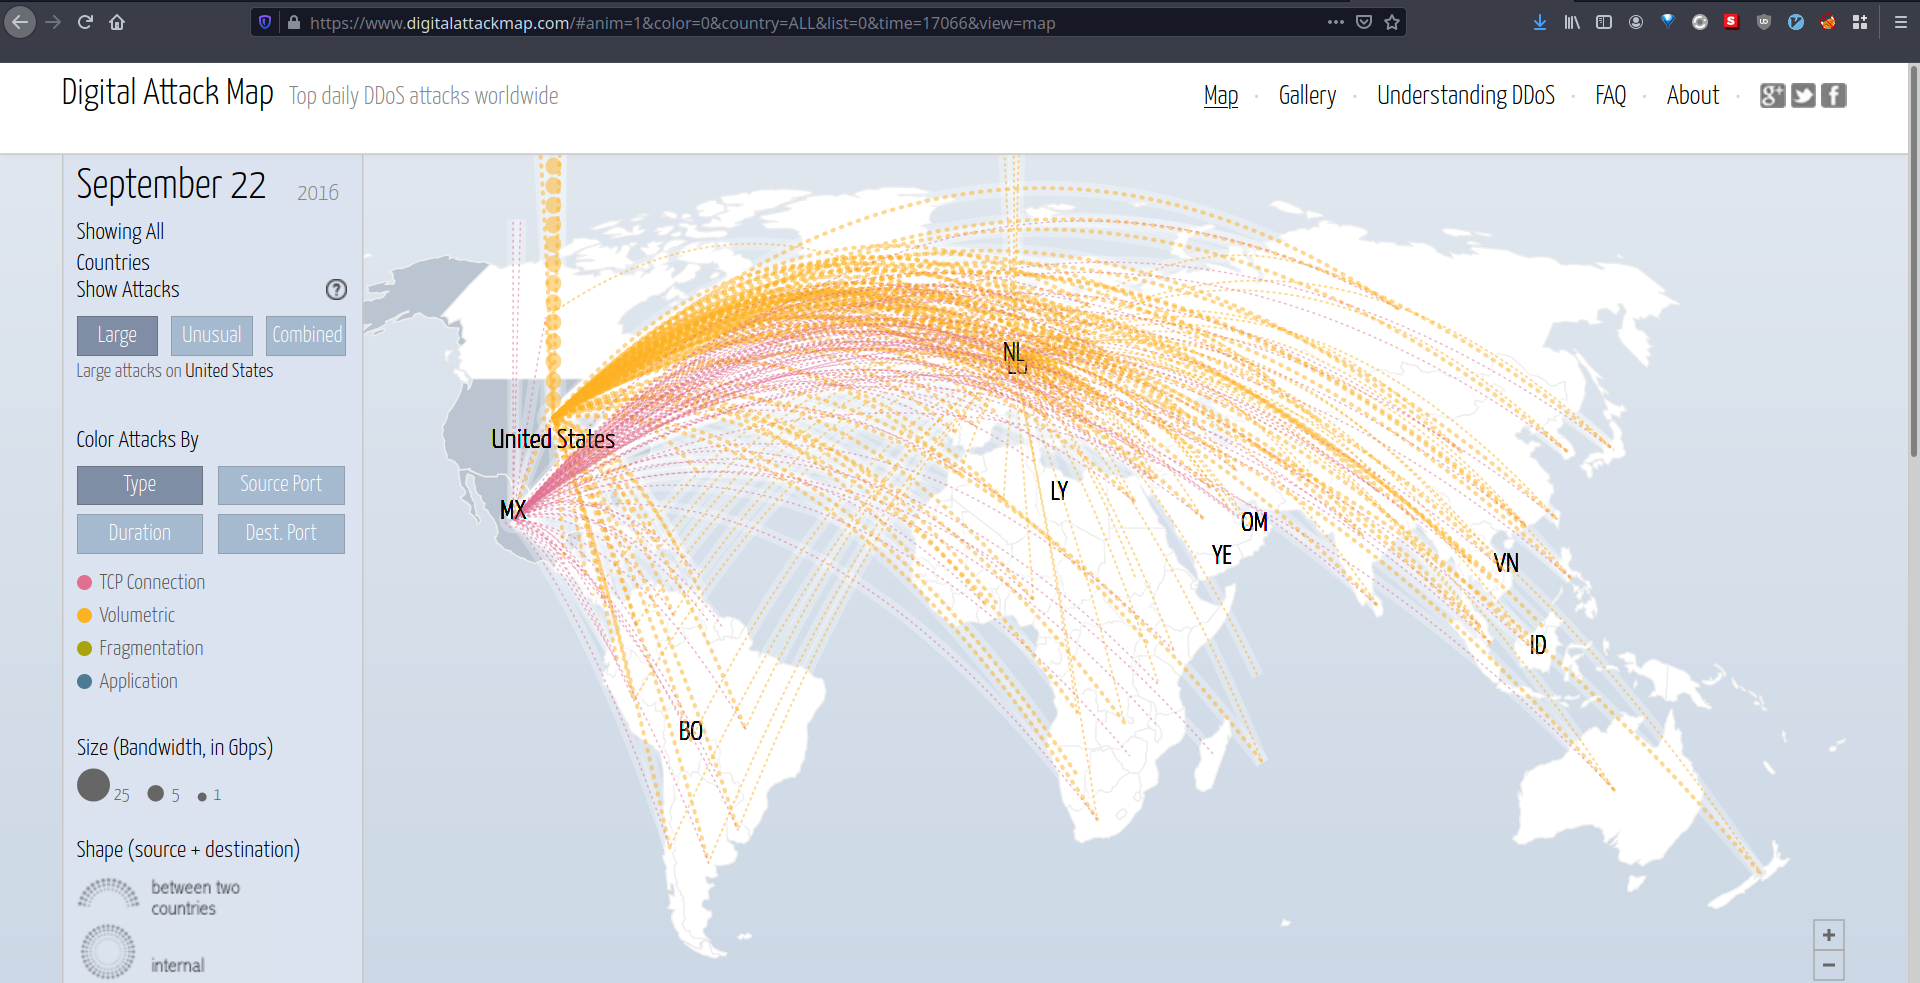
\includegraphics[width=\linewidth]{images/kreb-on-security.png}
    \caption{Mirai DDoS to KrebsOnSecurity}
    \label{fig:mirai-ddos}
\end{figure}

Necurs was one of the largest botnets. It was involved with elite cybercrime groups, and performed different tasks: email spam, spread Dridex (one of the most devastating banking trojans), DDoS attacks, distributions of ransomware, distribution of scam emails among others \footnote{Necurs activities: \url{https://securityintelligence.com/the-necurs-botnet-a-pandoras-box-of-malicious-spam/}}. This botnet has been such a problem that Microsoft has taken action into stopping its progress this year \footnote{News about Microsoft efforts to stop Necurs: \url{https://www.newkerala.com/news/2020/40405.htm}}. Necurs had four million victims in 2016, and it has nine million nowadays; its growth has been humongous. Necurs has been successful thanks to its resiliency. It uses a Kernel Mode-Rootkit to get undetected by viruses, hide, and make it hard to remove. It has a modular architecture that allows flexibility, so developers of the botnet can adjust it depending on the use case (e.g., sending spam, distributing malware, making DDoS attacks, etc). It came with antivirus detection systems and a Domain Generator Algorithm to generate their Command and Control server domains. All these features make it successful.

\begin{figure}
    \centering
    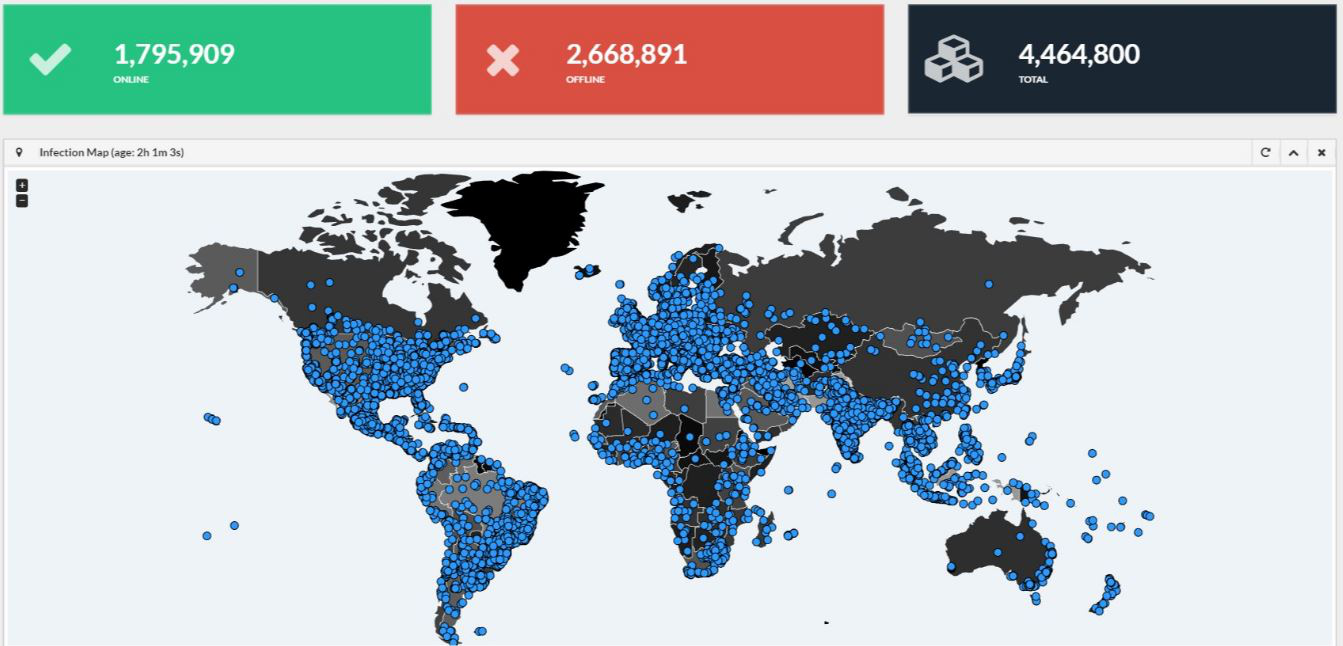
\includegraphics[width=\linewidth]{images/necurs-size.png}
    \caption{Number of infected machines by Necurs botnet. Reprinted from Security Affairs \cite{necurs-size}.}
    \label{fig:necurs-size}
\end{figure}

Internet of Things (IoT) opens the door to a new marvelous word, where all devices are connected. If just with computers cybercriminals could do Necurs, what will they do with all the devices that IoT is offering us? A new botnet more sophisticated which targets a wide range of devices thanks to IoT appeared in 2018, Torii. The best feature of this botnet, from our point of view, is that it uses Tor for his communications. Therefore, making it harder to know the origin. Moreover, it uses multi-level encryption of communication for its Command and Control architecture. Besides, it has six ways of gaining persistence in the system. Therefore, increasing its probabilities to stay on the computer \footnote{More info on Torii: \url{https://blog.avast.com/new-torii-botnet-threat-research}} \footnote{Torii video explanation: \url{https://www.youtube.com/watch?v=BjR6GwAGYDM}}.

Botnets could have seemed harmless before, but once you take a deep breath inside this area you realize that they can have an enormous big impact.

\chapter{Solution}
\label{solution}

We have seen various botnets with resilient design and interesting features. We are going to implement a similar botnet to Necurs, changing its architecture to P2P and implementing communication through Tor like Torii. This will add resiliency to the design, and make it harder to connect the botnet to our person (i.e, the attacker). Furthermore, we will implement a Kernel Mode-Rootkit to hide the malware (like Necurs).

\begin{figure}
    \centering
    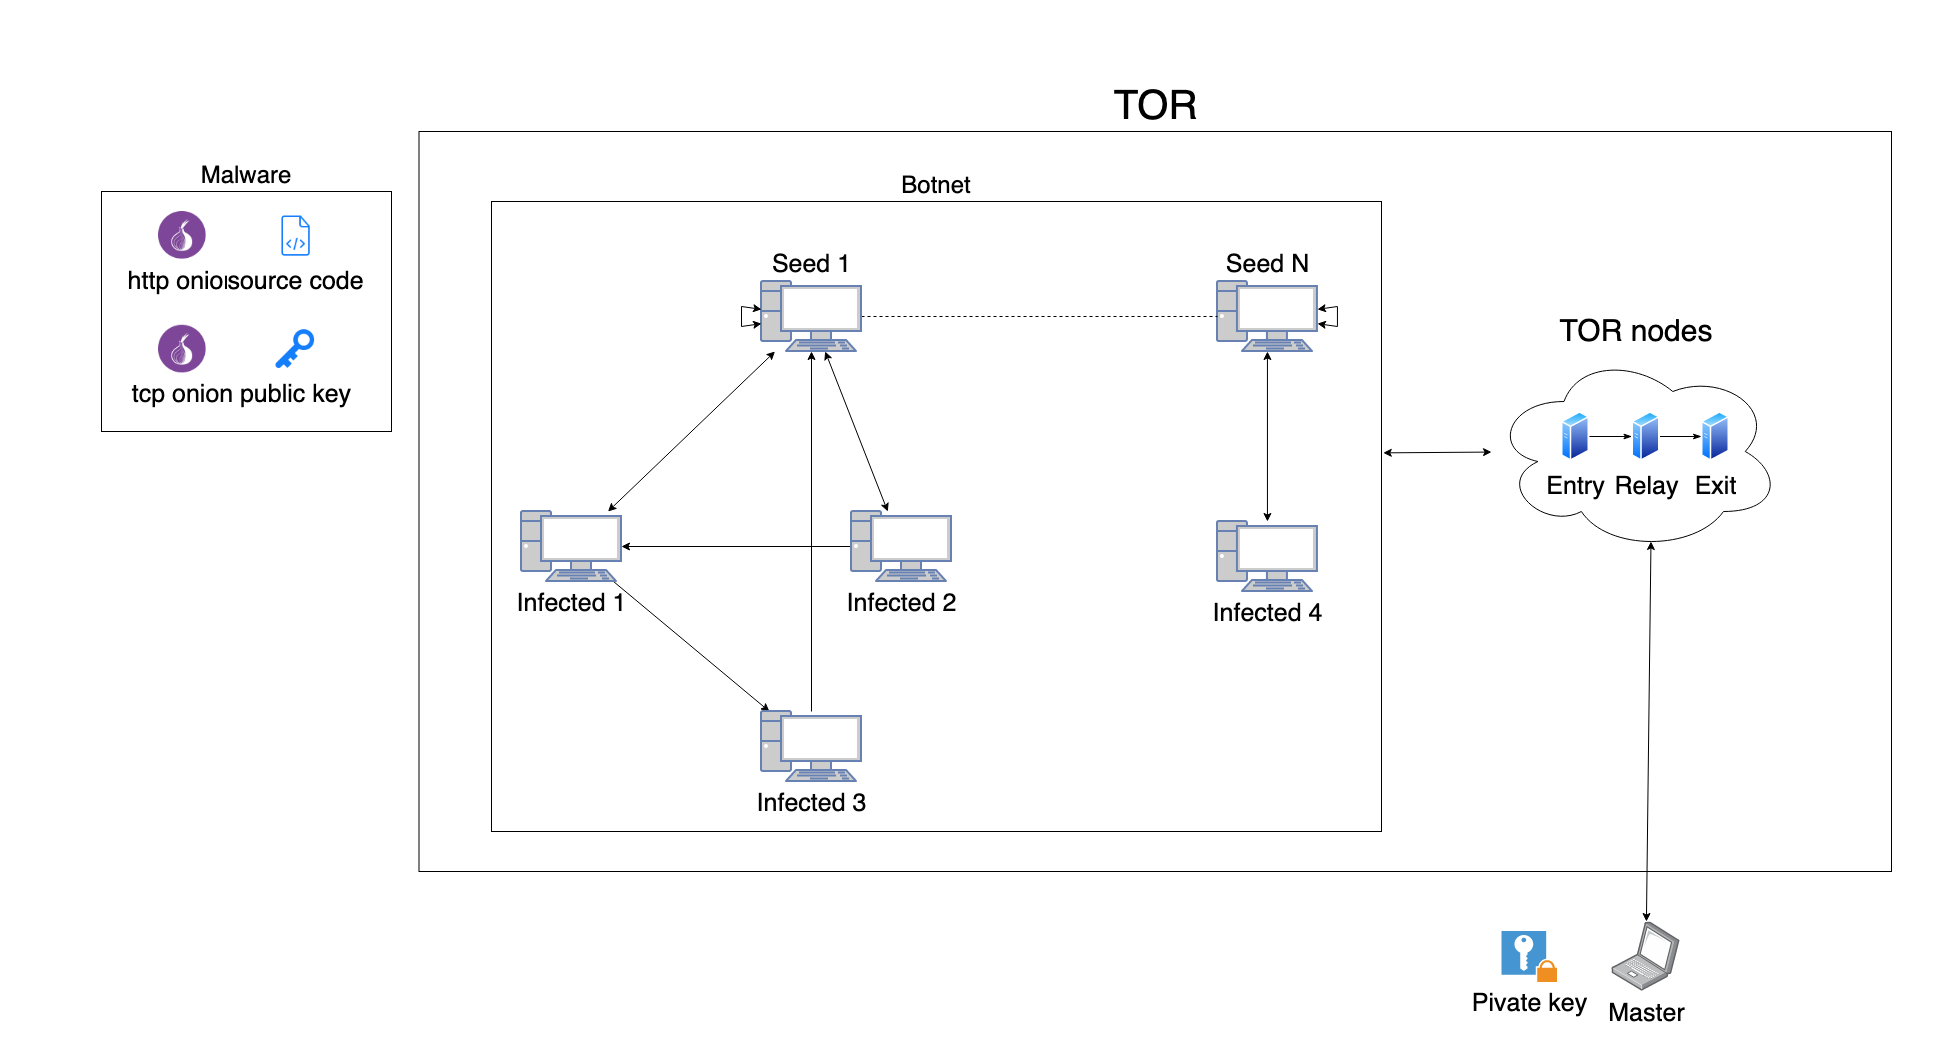
\includegraphics[width=\linewidth]{images/architecture.png}
    \caption{Botnet architecture and components}
    \label{fig:botnet-architecture}
\end{figure}

The basic architecture can be seen in figure \ref{fig:botnet-architecture}. The different elements are:
\begin{itemize}
    \item \textbf{Master machine:} Computer used by the master to access the botnet.
    \item \textbf{Private key:} Key only in the attacker possession to access the botnet.
    \item \textbf{Seed machine:} Attackers first "victims" prepared by the master.
    \item \textbf{Victim machine:} Machines of unknown people that get infected.
    \item \textbf{Malware:} Each victim and seed has a download and communication server so that peers can talk with each other and download files. Besides, a public key paired with the attacker's private key and the source code of the malware.
    \item \textbf{Tor network:} Open source anonymous network to improve communication anonymity between peers in the network.
\end{itemize}

The main idea is to create a network of victim machines using GNU/Linux systems that we (i.e., the attacker) will we able to access at any given time, knowing that only we can access the botnet and its victims. We will be able to execute commands on any victim machine and receive the response, besides being able to update it at will while the Kernel Mode-Rootkit hides the malware trace in the system. Moreover, all the communications will go through Tor to make it harder for the authorities to track the origin of the requests (i.e., the attacker).

The full code is in \url{https://github.com/danielorihuela/p2p-botnet}.

To better understand how the different elements in the architecture interact between them, we are going to explain more in detail the steps that are followed when infecting a machine, and when executing a command.

Trying to infect a new victim, that is not yet in the botnet using a computer not linked to the master of the botnet:
\begin{enumerate}
    \item Send fraudulent email to the victim with a file attached, from a computer not directly linked to the master of the botnet.
    \item Victim trust the email and opens the file, it starts sending messages through Tor to a seed machine
    \item If the seed is alive, the communication begins
    \item The infected machine downloads the files and sends to the seed its new onion directions created, besides the user name
\end{enumerate}

\begin{figure}[H]
    \centering
    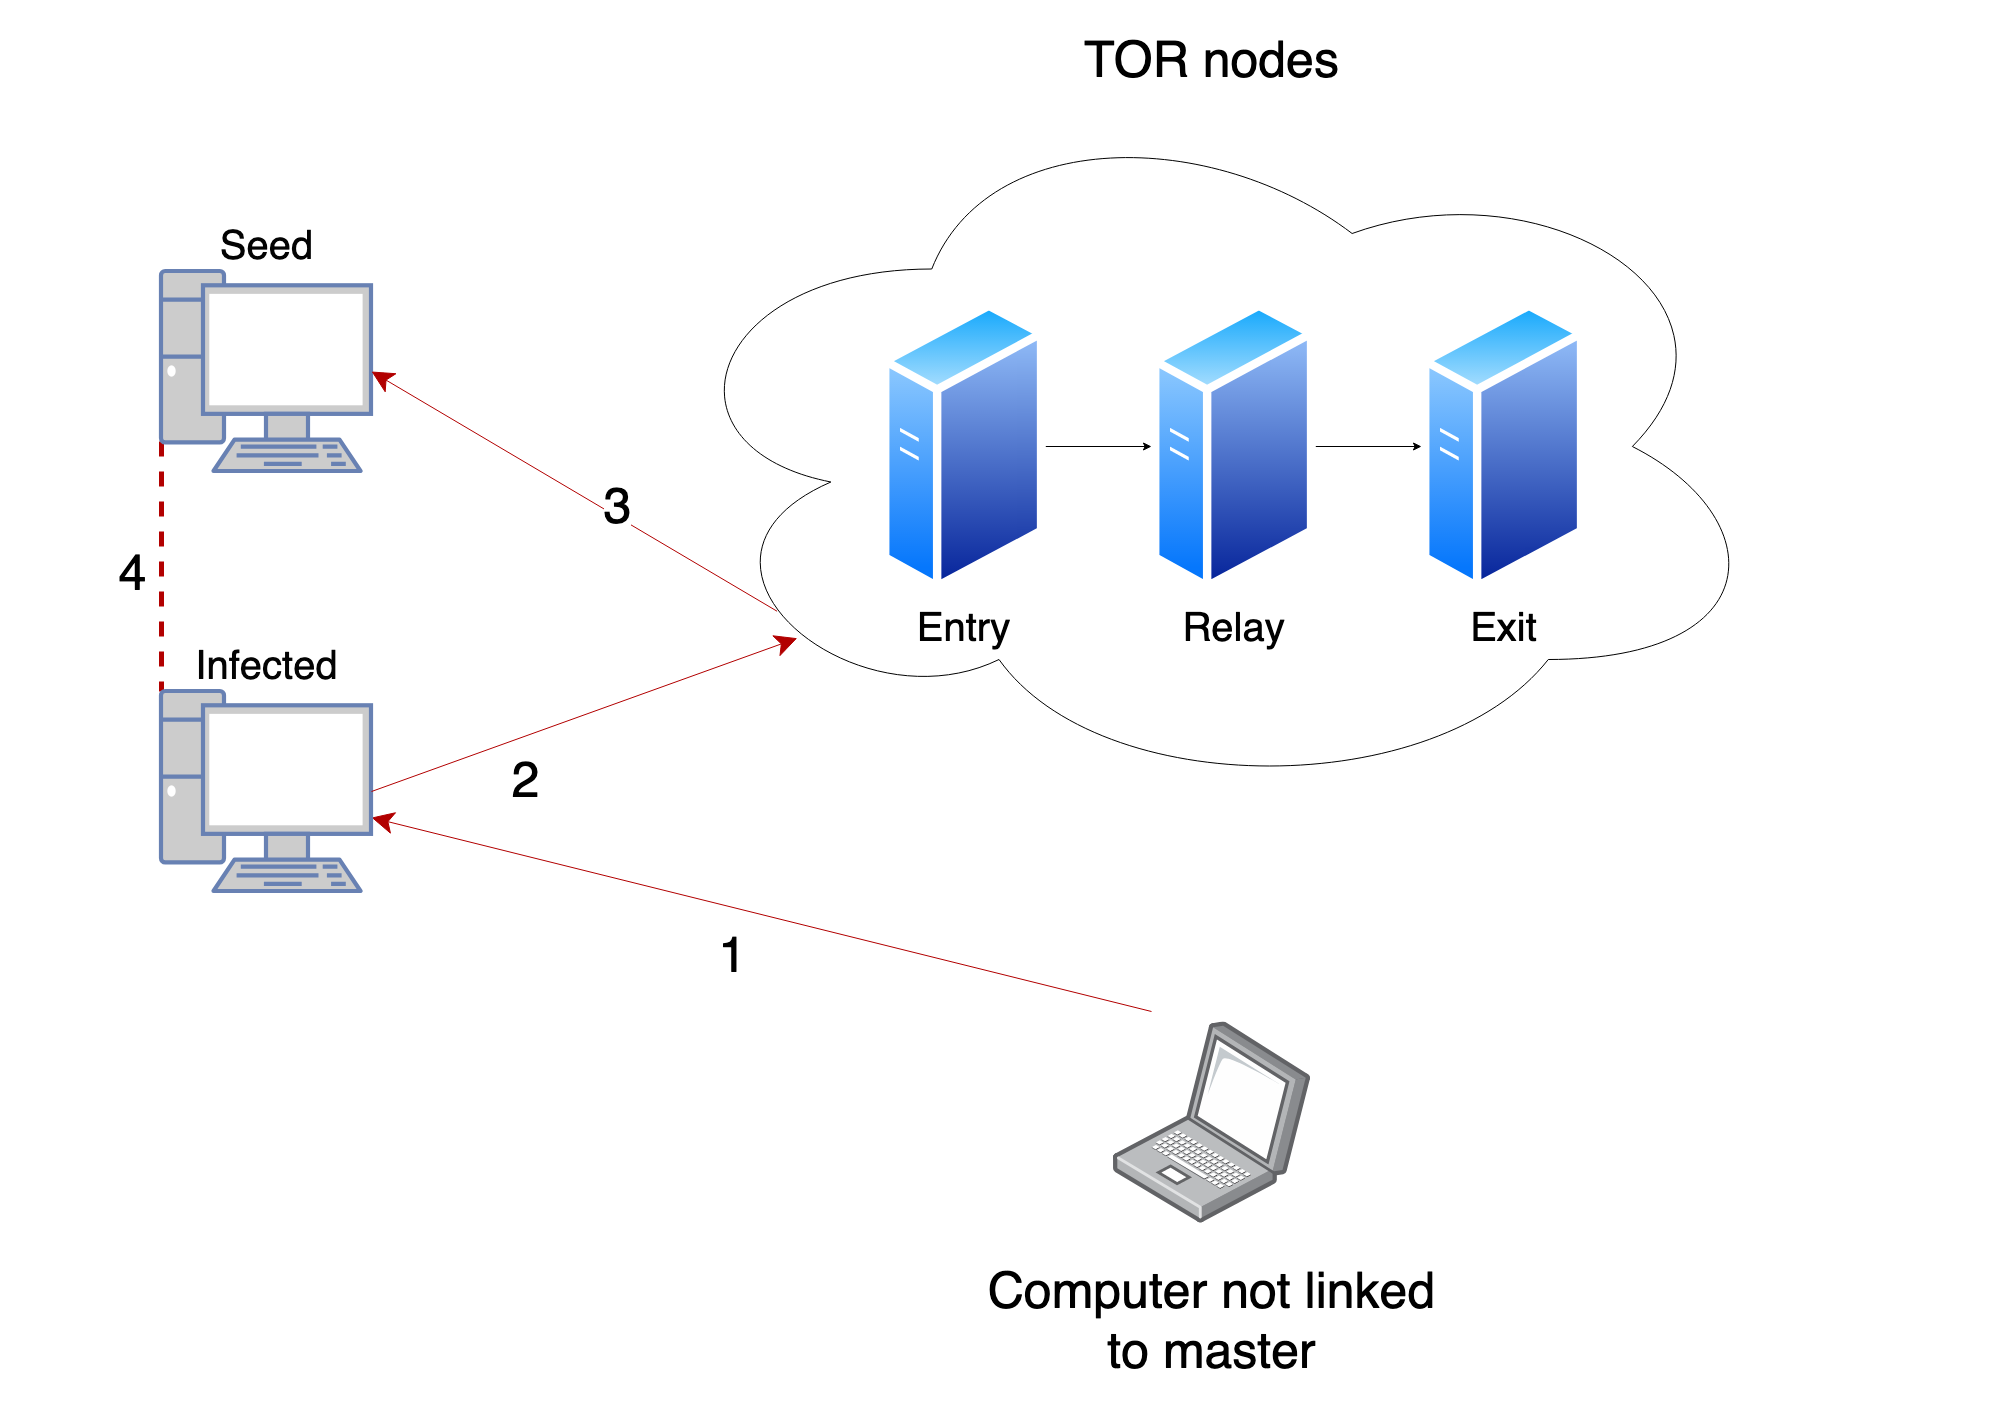
\includegraphics[width=\linewidth]{images/zoom.png}
    \caption{Infection protocol triggered by malicious file attached in email}
    \label{fig:botnet-architecture}
\end{figure}

As you can see, we infected a machine in just four steps and nodes are symbolically linked to each other (i.e., in step 4 nodes stored each other's information).

Now, the victim machine is at the attacker's mercy. The master can get any information he wants from the victim, even though it has to be done manually. That means the master has to connect to the victim and execute commands to get information. We can see the protocol it follows in the next steps.

\begin{enumerate}
    \item The attackers requests connection to the victim and executes a command
    \item The victim machine receives the message and checks it is signed by the master
    \item Sends the response to the master
    \item Receives the information
\end{enumerate}

These are the basic steps. Nevertheless, anonymizers can be used. In that case, some steps between steps 1 and 2 would be performed (1.5a and 1.5b) where the information flows to a middle victim machine before going to the final victim machine. The idea is that the message hops through different machines before reaching the final destination, and the response follows the same path backward. Due to the implementation of the botnet, the message sent by the attacker is in clear text and signed. However, the response is sent encrypted (so that the cybercriminal is the only person in possession of that information).

\begin{figure}[H]
    \centering
    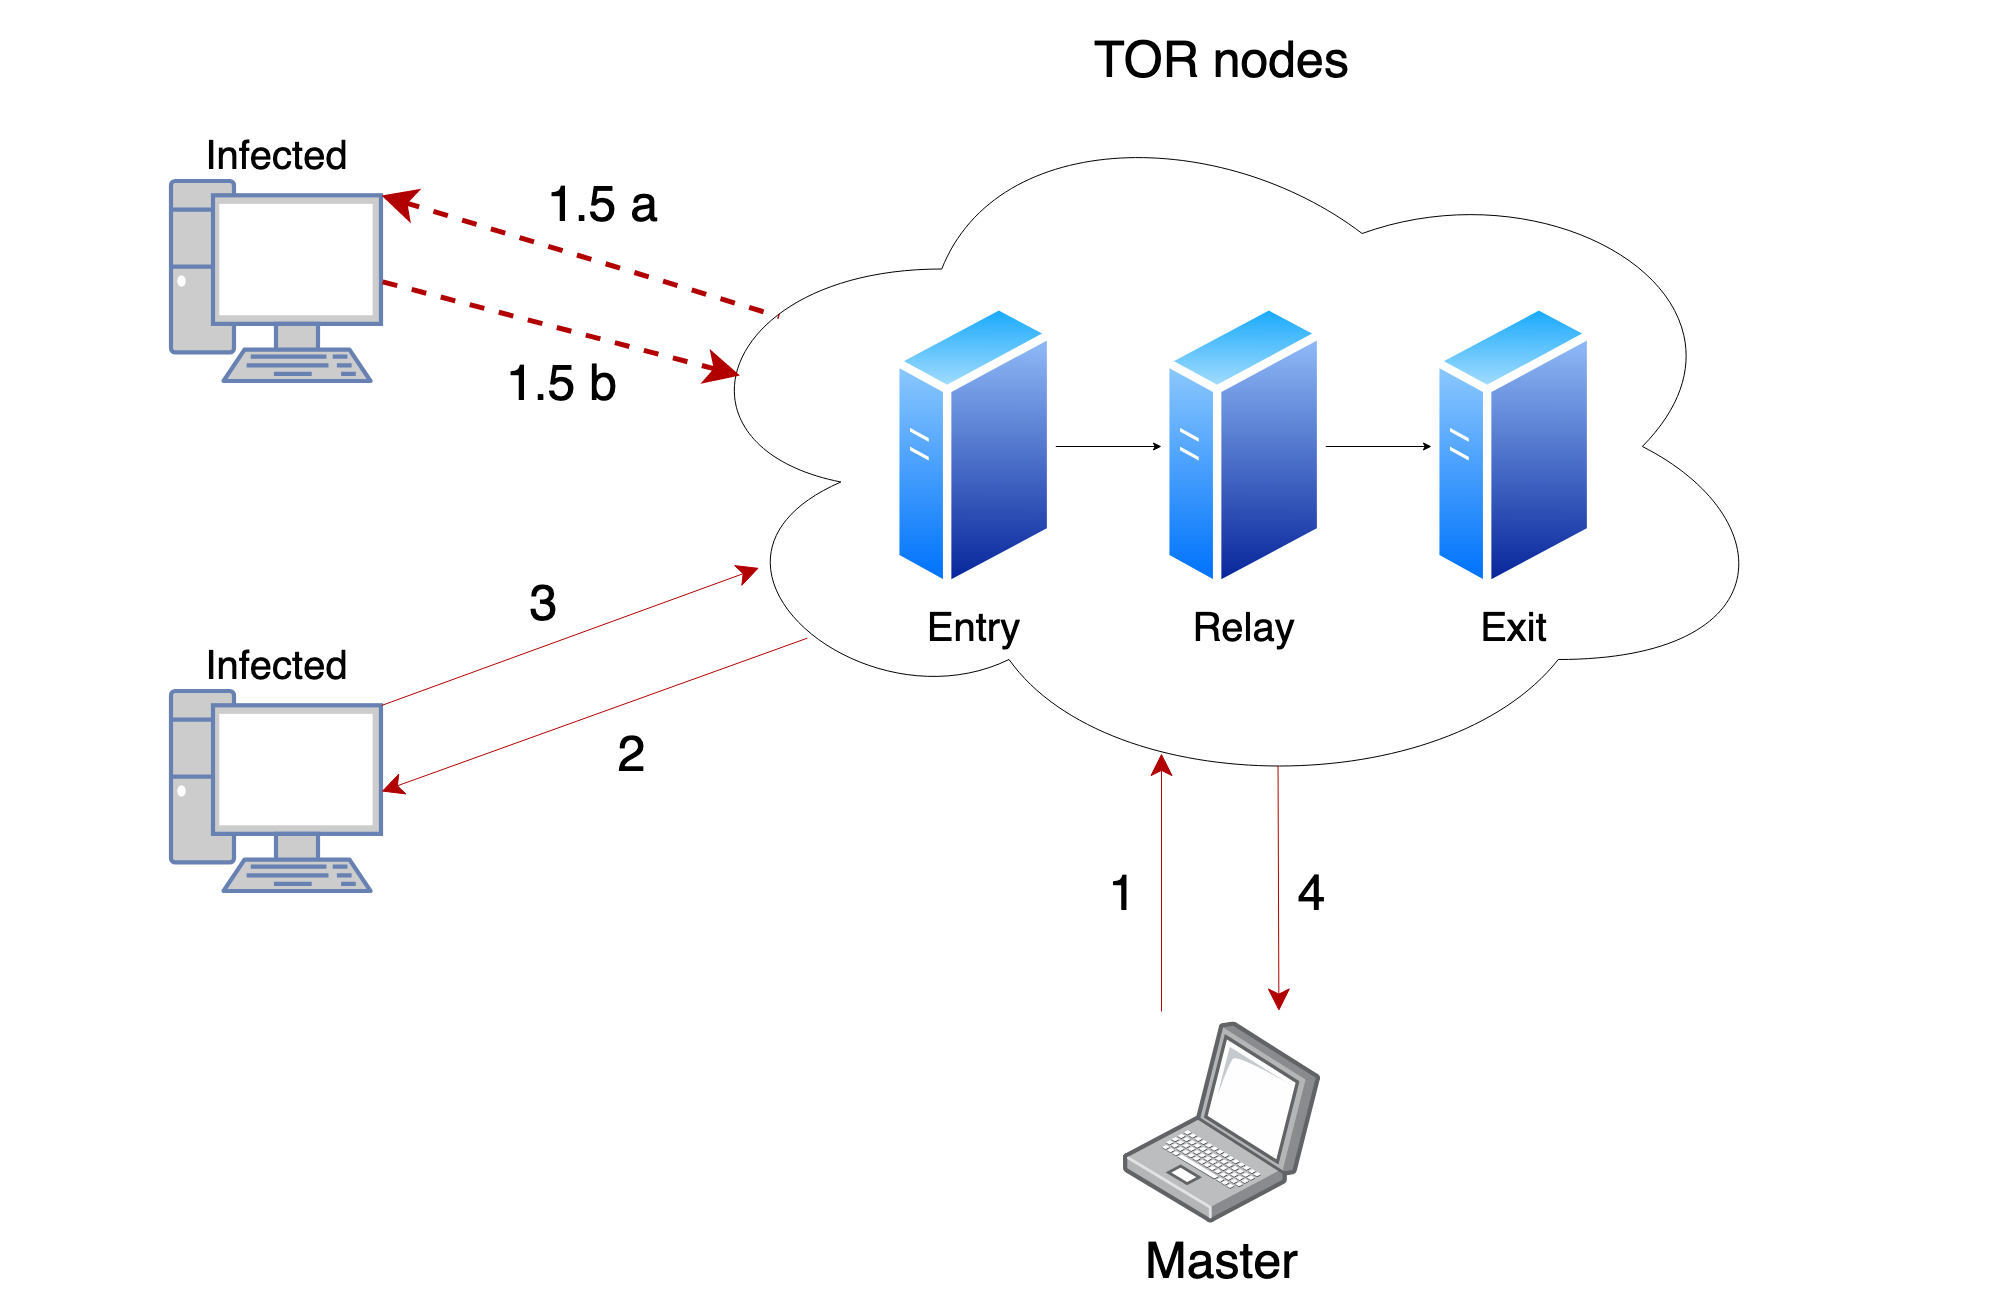
\includegraphics[width=\linewidth]{images/zoom-connection.png}
    \caption{Communication protocol when master executes a command}
    \label{fig:botnet-architecture}
\end{figure}

\section{Rootkit}

The first component we are going to discuss is the rootkit. The main goal of our rootkit is to hide the trace the malware could be letting behind (e.g., listening ports, files, folders, processes, logs, etc). Also, we want it to make the threat persistence across reboots.

Premise:
The victim machine is running GNU/Linux system. Specifically an Ubuntu distribution with kernel 5.3.0-45 generic.

Features:
\begin{itemize}
    \item Hide the LKM itself
    \item Hide the folder containing the malware. Taken from \cite{}
    \item Hide ports opened by the malware
    \item Hide processes started by the malware
    \item Persistence in the system
\end{itemize}

To implement all this we need to modify the victim machine at the user or the kernel level. For this, we can either create a user or kernel mode-rootkit so that we can hide things from the system. For the explanation, we assume you know C programming language and what pointers are.

In Linux, we can take advantage of the LD\_PRELOAD to create a user mode-rootkit. In Linux we have "shared libraries" (i.e., files to be used by different executables and other objects), and a "dynamic linker", which copies the content of the shared libraries from storage to RAM at runtime, so executables can work properly. LD\_PRELOAD is an optional environment variable where we can store one or more paths to shared libraries or shared objects, these libraries will load before any other shared libraries (i.e., we can create a program and preload it to modify the current behaviour of the system). We have a simple program that prints random numbers. By exploiting the LD\_PRELOAD trick we can change the current behaviour into printing always the same number.

\begin{figure}
    \centering
    \subfloat[Random numbers]{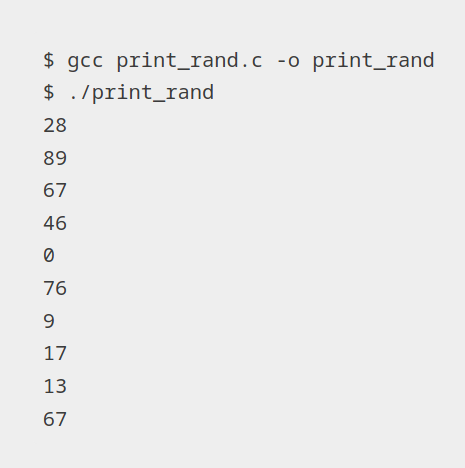
\includegraphics[width=5cm]{images/random-numbers.png}}
    \qquad
    \subfloat[Random numbers modified with LD\_PRELOAD]{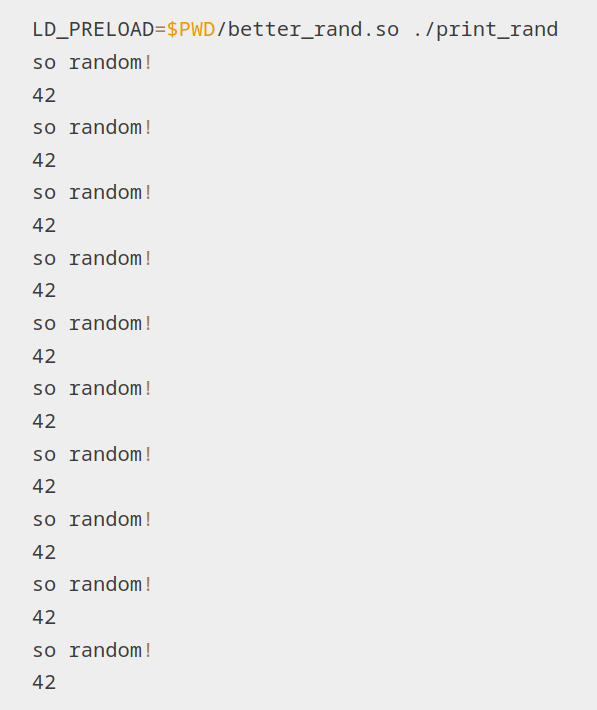
\includegraphics[width=5cm]{images/not-so-random.png}}
    \caption{Code printing random numbers before and after using LD\_PRELOAD. Reprinted from The Meta Bytes \cite{ld-preload-trick}.}
    \label{fig:random-numbers}
\end{figure}

This was our first approach to the rootkit. However its main drawback is that it is running at the user level, therefore it is easy to detect and to remove. For this reason, we gave up on this and moved on to the kernel mode-rootkit.

Kernel mode-rootkit is better, once we infected a machine we are at the same level as the kernel, so we can modify it to lay low, and keep undetected even by antivirus. In Linux, we have two ways to do this. The first one is to modify the kernel and expecting that the user installs this modified OS on his computer. The second one is a better option, we just need to create an LKM and expect the user loads it into its kernel. The first approach gives more problems since you have to make the user install a new and complete OS into his system, very unlikely. For this reason, we decided to use an LKM for our rootkit, which is easier to trick the user into installing or to download the code when the user uses some software with a vulnerability.

Deciding factors:
\begin{itemize}
    \item Small size
    \item Easy to inject into the system
    \item Exists at the kernel level
    \item Modify the kernel behaviour
    \item Better tool to hide from the kernel
\end{itemize}

We already discussed what an LKM is in section \ref{loadable-kernel-module}. Now we will see how we can take advantage of it in Linux to hide the malware.

The first step is to hide the LKM itself. Linux stores the information about modules in two VFS, /proc (mainly contains information about processes) and /sys (stores information about system-level files and properties). Therefore, we must delete the information from both of the VFS. See figure \ref{fig:hide-lkm}.

\begin{figure}
    \centering
    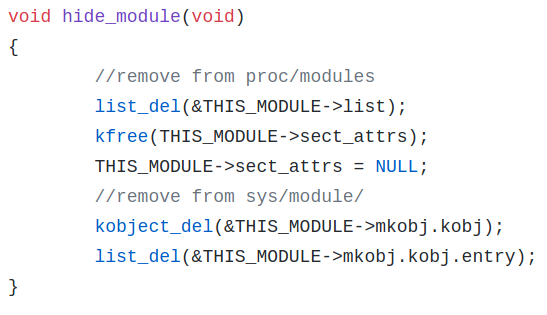
\includegraphics[width=\linewidth]{images/hide-lkm.png}
    \caption{Function to hide LKM}
    \label{fig:hide-lkm}
\end{figure}

The second step is to hide the folder where our malware will live. We will use strace, a command-line tool used for debugging interactions with the system kernel in Linux. It monitors system calls and signals.

\begin{lstlisting}
$ strace ls
[...]
openat(AT_FDCWD, "/proc/filesystems",
        O_RDONLY|O_CLOEXEC) = 3
[...]
getdents64(3, /* 99 entries */, 32768)  = 3312
[...]
\end{lstlisting}

After issuing the above command, we can see that one of the printed lines contained a function called getdents64. It turns out that getdents64 is a system call which you can use to get the directory entries, so we can modify this function to remove a folder from the list. The other line tells us that at some moment, the /proc VFS is opened. 

/proc VFS has a structure containing a pointer to "file\_operations", another structure with some operations as we can see in figure \ref{fig:proc-dir}. We can see the Linux kernel source code in the "bootlin" webpage (\url{https://elixir.bootlin.com/linux/latest/source}).

\begin{figure}
    \centering
    \subfloat[proc\_dir\_entry structure]{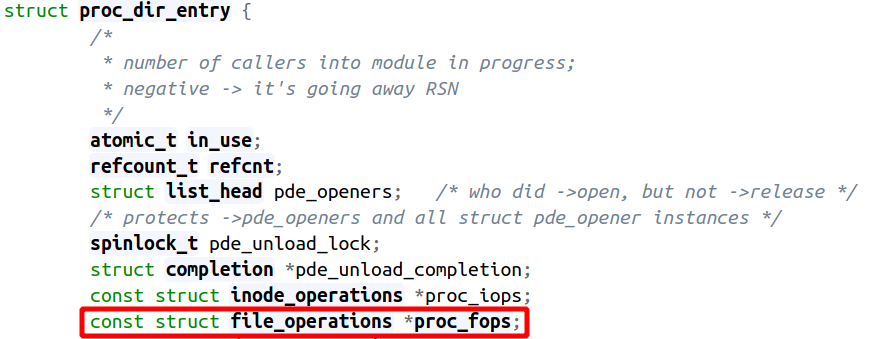
\includegraphics[width=6cm]{images/proc_dir.png}}
    \qquad
    \subfloat[file operations structure]{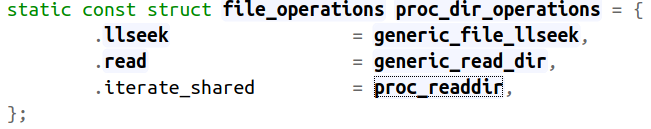
\includegraphics[width=5cm]{images/fops.png}}
    \caption{Linux 5.3.0 source code.}
    \label{fig:proc-dir}
\end{figure}

If we return to getdents64. We can see that it executes ksys\_getdents64, which calls iterate\_dir, which calls iterate\_shared. As we have seen, iterate\_shared can be reached from both the proc\_dir\_entry and getdents64, by modifying it we will be able to hide a folder. One of the parameters iterate\_shared receives is a dir\_context struct pointer, which contains a pointer to a function called filldir\_t, used by the readdir() to let the kernel chose the layout needed when printing the information.

\begin{figure}
    \centering
    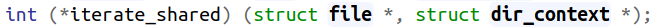
\includegraphics[width=\linewidth]{images/iterate-shared-prototype.png}
    \caption{Iterate shared arguments in Linux kernel 5.3.0}
    \label{fig:scheme-hide-folder}
\end{figure}

\begin{figure}
    \centering
    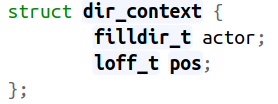
\includegraphics[scale=0.6]{images/dir-context.png}
    \caption{dir context struct in Linux kernel 5.3.0}
    \label{fig:scheme-hide-folder}
\end{figure}

\begin{figure}
    \centering
    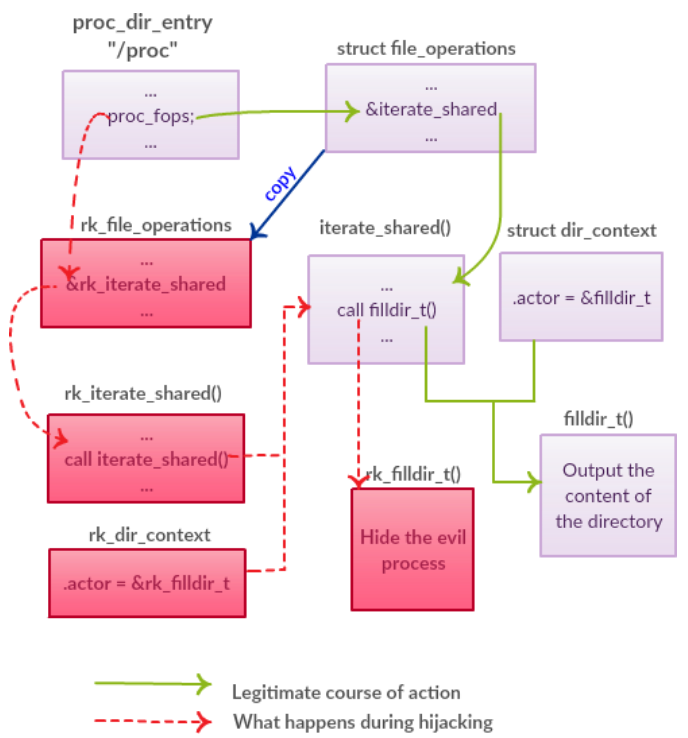
\includegraphics[width=\linewidth]{images/root-map.png}
    \caption{Hijack Linux kernel scheme to hide folders. Reprinted from yassine.tioual.com. \cite{rootkit-folder}}
    \label{fig:scheme-hide-folder}
\end{figure}

\clearpage
To summarize before continuing, in figure \ref{fig:scheme-hide-folder} we can see all the previously mentioned functions and structs that come into play when we want to hide a folder. proc\_dir\_entry has a pointer to a file\_operations struct that has a pointer to an iterate\_shared struct. This iterate\_shared points to a function called filldir\_t, that modifies the layout when printing information. Therefore, by modifying this function we can modify the folders printed when executing a command in the shell. We want to hide all files and folders starting with a specific prefix. In figure  \ref{fig:hide-folders-files} we show our function. We check if the received file name (remind that in Linux all can be treated as a file, folders too) starts with the prefix. If that is the case we return 0 to hide it, otherwise we return the output of the original function. After changing the pointers from the structures as indicated in figure \ref{fig:scheme-hide-folder}, we successfully hijacked filldir. As a result, we can hide folders and files from any VFS in the system. We can see a little demo in figure \ref{fig:filldir-hijacked-demo}; where the files and directories are not shown, but if you know their location you can see their content.

\begin{figure}
    \centering
    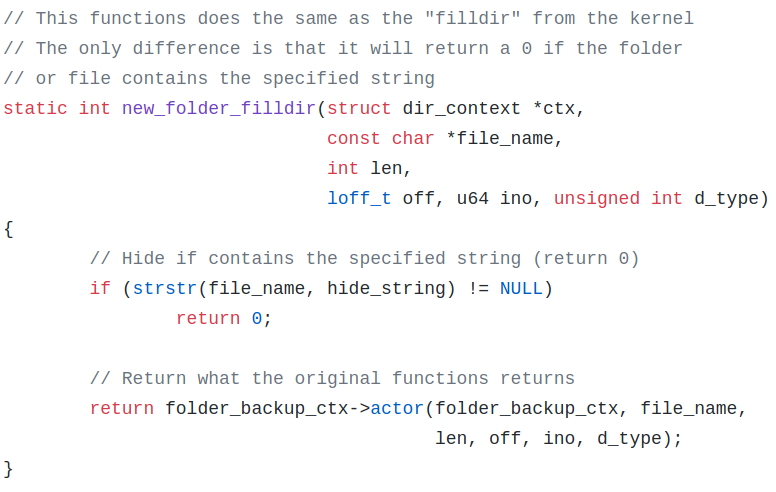
\includegraphics[width=\linewidth]{images/hide-folder-code.png}
    \caption{Modified filldir to hide folders and files}
    \label{fig:hide-folders-files}
\end{figure}

\begin{figure}
    \centering
    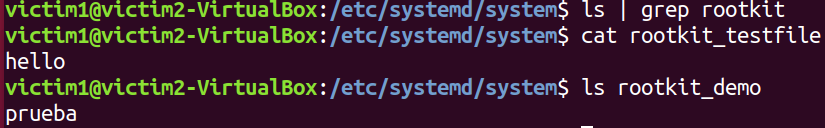
\includegraphics[width=\linewidth]{images/hide-example.png}
    \caption{Hide files and folders demo}
    \label{fig:filldir-hijacked-demo}
\end{figure}
\newpage
Process information is stored in /proc VFS as well, so we only need to change the filldir to hide processes. It is a large function, but the important part can be seen in figure \ref{fig:filldir-hijacked-proc}. We have a file called "process" where we store all the processes pid (i.e., process identifier) we want to hide. When calling filldir we return 0 if the number is stored in the file. Otherwise, we return the original output. Figure \ref{fig:filldir-hijacked-proc-demo} shows a little demo.

The implementation of the code is based on the Github repository of a guy who also explained the process of hijacking the filldir function on his blog \cite{rootkit-folder}. Both features: hiding processes and folders come directly from his repository. We just modified the hiding process feature, to hide all processes given a file with the process identifiers.

\begin{figure}
    \centering
    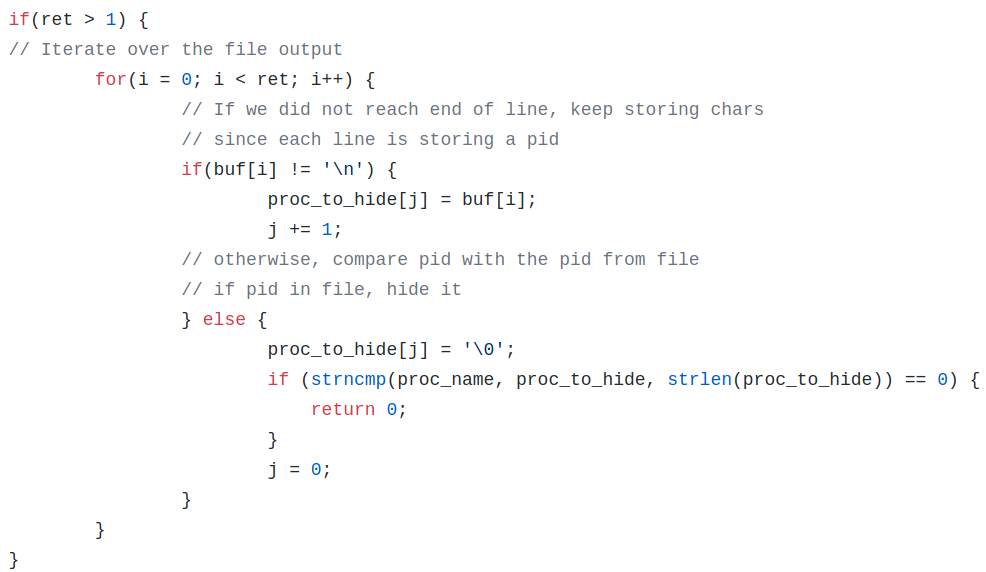
\includegraphics[width=\linewidth]{images/hide-proc-fopr.png}
    \caption{Modified filldir to hide processes code}
    \label{fig:filldir-hijacked-proc}
\end{figure}

\begin{figure}
    \centering
    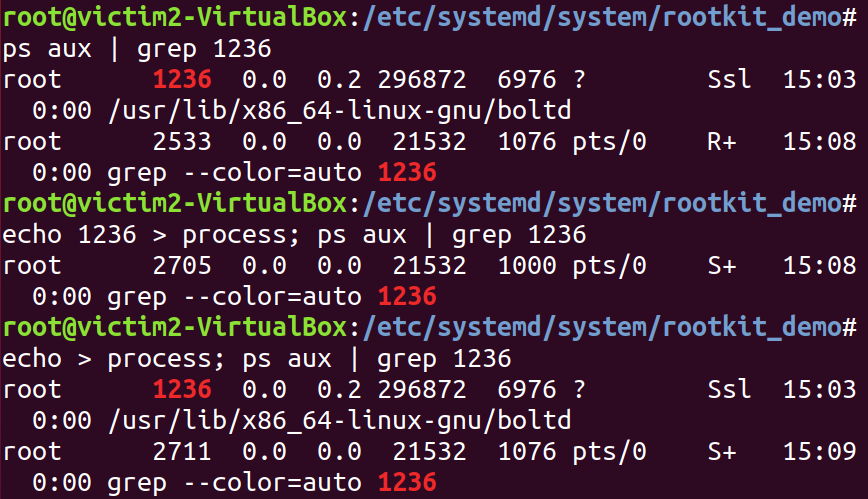
\includegraphics[scale=0.5]{images/hide-process.png}
    \caption{Hide processes demo}
    \label{fig:filldir-hijacked-proc-demo}
\end{figure}
\newpage
Our rootkit hides itself, folders, and files. Furthermore, we added a feature to hide open ports from netstat.

\begin{lstlisting}
$ strace netstat -t
[...]
openat(AT_FDCWD, "/proc/net/tcp", O_RDONLY) = 3
[...]
\end{lstlisting}

We execute the above command to see how the command interacts with the OS. To list all the TCP ports the OS opens the /proc VFS to take the information. If you take another look to figure \ref{fig:proc-dir} you will see in the proc\_dir\_entry a pointer to seq\_operations. This struct is used various times in the kernel to know which tcp4, tcp6, and udp functions must be used.

\begin{figure}
    \centering
    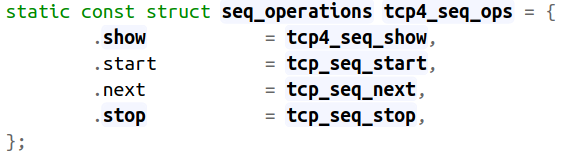
\includegraphics[scale=0.7]{images/tcp-seq-file.png}
    \caption{tcp4 operations}
    \label{fig:tcp-seq-file}
\end{figure}

The most interesting function in figure \ref{fig:protection_ring_figure} is tcp4\_seq\_show. Its responsibility is to show the ports. If we can get hold of that function, we will be able to hide tcp4 ports.

\begin{figure}
    \centering
    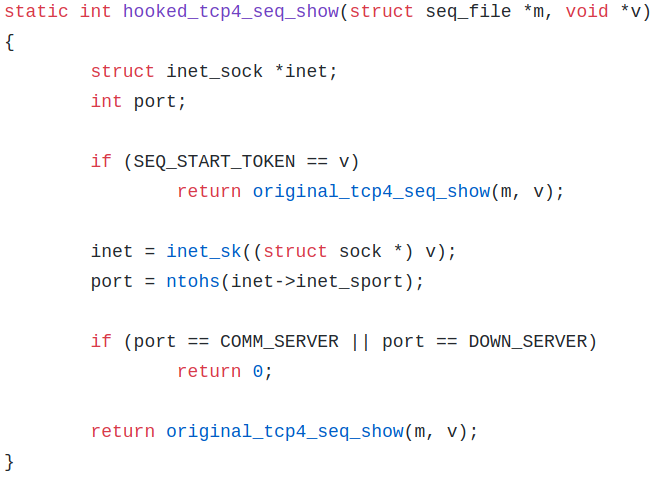
\includegraphics[scale=0.7]{images/tcp4-hooked.png}
    \caption{tcp4\_seq\_show modified}
    \label{fig:tcp4-modified}
\end{figure}

Now, we modify tcp4\_seq\_show to hide the ports we want. In our case will be the COMM\_SERVER and DOWN\_SERVER variables as we can see in figure \ref{fig:tcp4-modified}. The result of introducing an LKM to the kernel with that change is that when listing the ports some of them will not appear. We can see the example in figure \ref{fig:hide-from-netstat}.

\begin{figure}
    \centering
    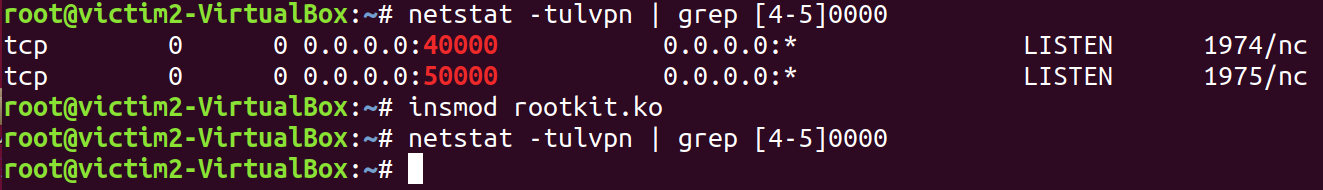
\includegraphics[width=\linewidth]{images/hide-ports-from-netstat.png}
    \caption{Hide ports from netstat demo}
    \label{fig:hide-from-netstat}
\end{figure}

Our rootkit is now prepared to hide all traces from the infected computer. We must think now on how do we infect a victim and which architecture are we going to use.

\section{System Architecture}

We already discussed the different types of botnets, its advantages and disadvantages in section \ref{section:botnets}.

We decided to use a full P2P botnet architecture, as it gives us resiliency against our adversary (e.g., the Government) attacks to shut down the botnet (i.e., we have lots of servers, not only one Command and Control server). Even though it has some bottlenecks.

Premise:
Once a node is infected, it will remain alive at all times; nodes will not disjoin never the network (i.e., the malware will not be removed from an infected machine).

Features:
\begin{itemize}
    \item Execute commands in victim machines and receive output
    \item Update malware files
    \item Use victims as anonymizers to connect to other victims
    \item Use Tor for communications
\end{itemize}

\subsection{Botnet bootstrap and spreading}
Figure \ref{fig:botnet-architecture} shows our botnet once is built, but not the process. We need to bootstrap the botnet, so we build from the ground up a seed machine (i.e., a victim machine made by ourselves), where the first real victims will connect. From there, the idea is to manually include some of these machines to the script that infects the victims. To do this you must keep control of victims: is the victim connected? did the victim remove the malware? will he return?... All this must be handled to make a resilience botnet, for us this will be simplified due to the previously mentioned premise. Given enough time, we would have a P2P botnet with a large enough list of machines where new victims can connect.
\newpage
Malware researches investigate botnets among others. One of the things they do is estimate the size of the botnet. Most of the time botnets do not take this into account and allow access to all peers from a single victim, given that it is a P2P or hybrid botnet. To lessen the accuracy of the size and increase the required time to make the prediction we implemented two lists of nodes instead of one like every botnet we investigated do. Each machine has a private peer list with all the machines that connected to him when infected, and a public peer list containing a subset of two machines from the private peer list. Only the master can see the content in the private peer list, besides the victim itself. Before moving on, we need to understand the protocol to add new victims to the botnet.

Protocol:
\begin{enumerate}
    \item Victim gets infected.
    \item Sends required information to selected peers (i.e., node from the hardcoded list of nodes).
    \item Selected peer saves the info in the private peer list.
    \item Selected peer chose at random one line of the public peer list (if it already has length 2) and overwrites it with the new peer data.
    \item Victim downloads the malware and all the required public files from the selected peer.
    \item Victim creates its private peer list from the downloaded public peer list.
\end{enumerate}

Anyone investigating the botnet will only have access to neighbours in the public list of any victim, plus neighbours in the private list of their infected machine. That means a long time to get every node, and it may be not the case. Since they only can see the public neighbours of the other victims, it may be the case where there is a computer that does not appear in any public peer list. This computer is unreachable for anyone except the master, who can access private peer lists. Similarly, we could end with clusters due to the above protocol. Imagine we have computer A, B, C, D, and E. Somehow, computers A and B are connected to C, computer C is connected to D and computer D is connected to E. At some point, a new computer F appears and uses computer C as a seed. Computer C reached the limit of lines in the public peer list, randomly it removes its connection to D. We could end with two clusters. One having computers A, B, C and F; and the second being of computers D and E. That way, the botnet could end up divided into clusters which are not accessible for a normal user, but it is accessible for the master user (i.e., the connections only exists in the private peer list, not the public one). That means that some parts of the botnet will remain hidden, potentially tricking the adversary that our botnet is not very powerful. To demonstrate this, we have done a small program that calculates the mean number of nodes with an indegree value of 0 in 100 experiments with botnets of 100 nodes simulating the above protocol. Moreover, we include graphs with and without clusters at the end of this section. The interesting thing about the botnet with clusters is that the adversary could end on a cluster with twenty nodes and not seeing the other eighty nodes.

To summarize, we are twisting the botnet reality into the eyes of the adversary. It is bigger than it may seem from the outside (e.g., looking at public peer lists), and it is very resilient thanks to the P2P architecture.

\begin{figure}
\centering
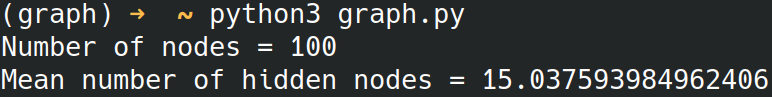
\includegraphics[width=\linewidth]{images/hidden-nodes-median.png}
    \caption{Mean number of hidden nodes}
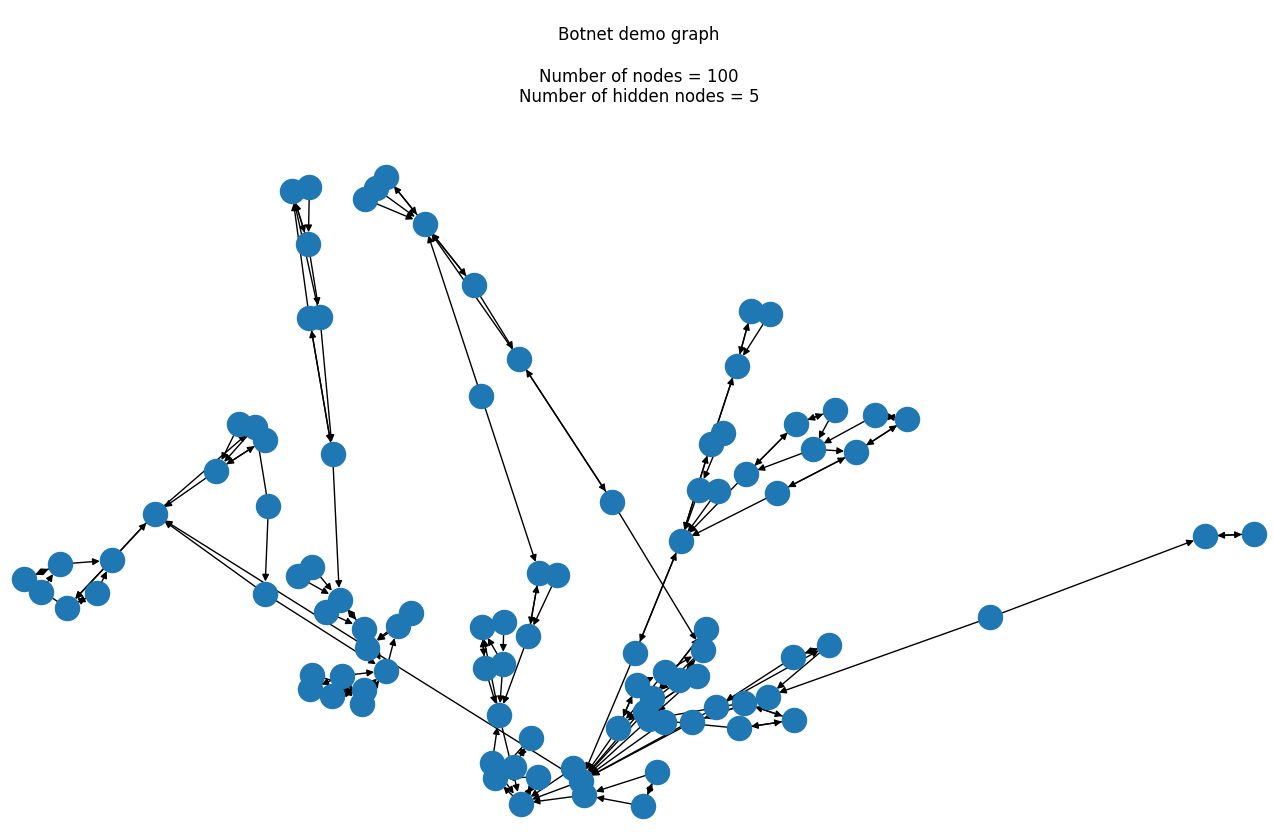
\includegraphics[width=\linewidth]{images/demo-graph-2.png}
    \caption{Botnet without clusters}
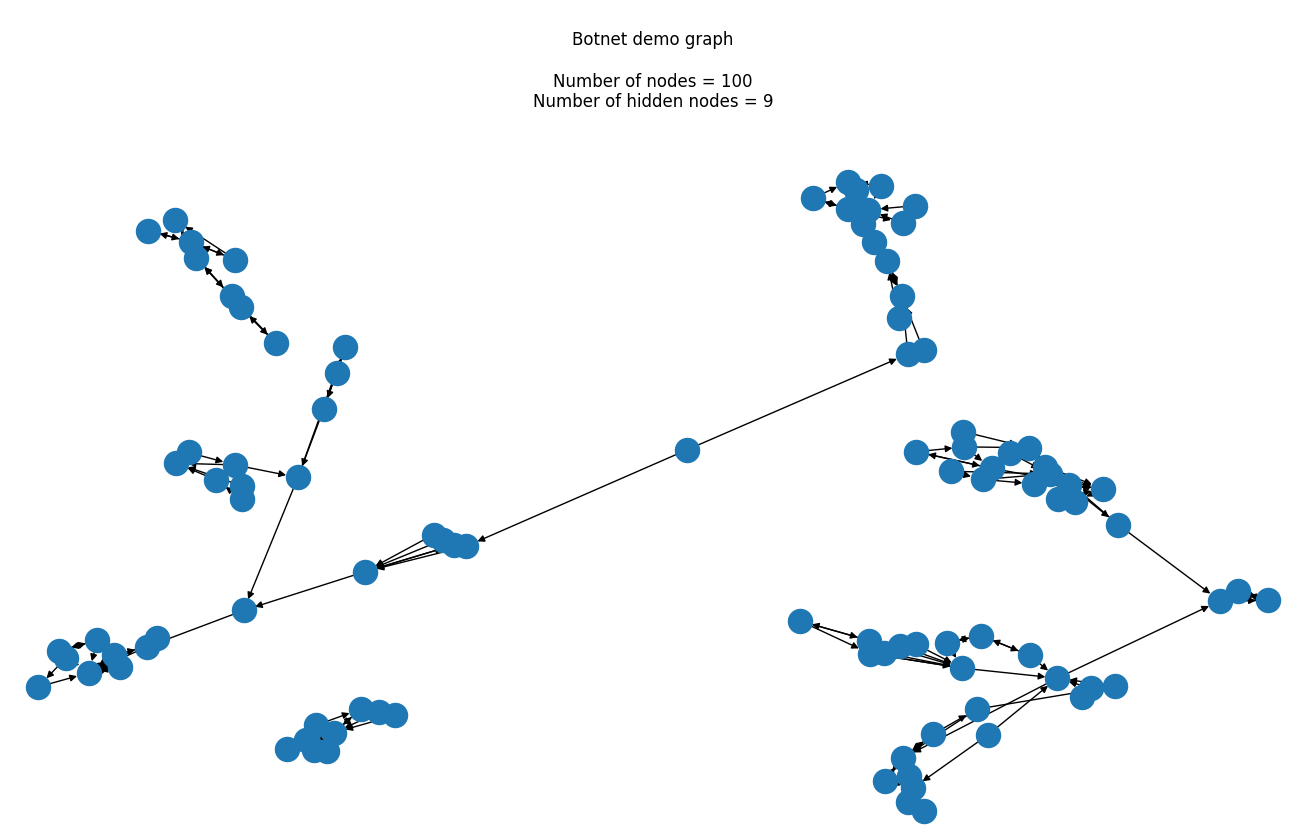
\includegraphics[width=\linewidth]{images/demo-graph.png}
    \caption{Botnet with clusters}
\end{figure}

\subsection{Botnet features}

We mentioned the features at the beginning of this section. We want to discuss how we have done them. Which types of security we implemented, and how these features work at a high level.

The first thing to understand is that we implemented asymmetric cryptography to the botnet. Every infected machine has a public key paired with the private key the master owns. Hence, only the person or group of people owning that private key can execute commands on victim machines and expect to receive an output, by signing the messages. That helps against third parties trying to steal our botnet, destroying it, or using its power for free.

Secondly, each infected machine has two onion services: one allows new victims to download the malware and all the required files, while the other allows communication through Tor between neighbours. Using onion services adds an encryption layer, it also hinders adversaries' efforts to know the real origin or recipient of the message. Nevertheless, some attacks can be done in Tor to deanonymize people and servers as we saw in section \ref{tor-attacks}. To avoid problems originated from attacks to Tor, we added the capability to use victim machines as anonymizers. We can put as many computers as we want, between us and the recipient. This hinders adversaries' effort to identify our real person. We mentioned in section \ref{path-length} that increasing the number of nodes in the middle does not help with security, the adversaries only need the first and last hops. It may seem this feature makes no sense. However, in our case we are not adding machines, we are adding circuits. To the best of our knowledge, correlation attacks do not take into account multiple circuits in a chain; even though they could. Assume for a moment that this kind of algorithm is possible and exists. Adding circuits to the chain means the adversary needs to own every pair of entry and exit nodes of each circuit used in our chain. Tor already made his three-node scheme knowing the odds of that are low. Using anonymizers lower these odds.

Finally, we have some basic features that allow us to get information from the victim and perform attacks. We can execute a command in the victim machine and receive its output and we can update a malware file.

To conclude, as you can see the botnet has few capabilities. Nonetheless, we want to show how a well-made botnet can: be resilient against attacks or takeovers, protect the master of the botnet, be flexible enough to add or update the current behaviour of the botnet, and at the same time partially hiding its real potential.

\section{Infection Vector}

The last piece of the puzzle if the infection vector. How do we infect victim machines more stealthily? How do we trick the user into installing the malware? To answer these questions you must know which types of users you are targeting. It is not the same to target windows than Linux users, and it is not the same to target people in Spain than people in Germany. You must think carefully which is the best you can do to get into your victim machine. For demo purposes, we have chosen a specific type of user and made some premises. We are going to target people with knowledge about GNU/Linux systems and vim (i.e., probably developers that use vim to edit text). Furthermore, we are supposing they are beginners or people with little security awareness. About the tooling, assume these people uses Vim 8.1.13.6 \footnote{Vim 8.1.13.6 vulnerability: \url{https://www.unix-ninja.com/p/exploiting_vim_with_cve-2019-12735}}, which will allow us to execute arbitrary code; and sudo version 1.8.21p2-3ubuntu1 \footnote{Sudo version 1.8.21p2-3ubuntu1 vulnerability: \url{https://blog.aquasec.com/cve-2019-14287-sudo-linux-vulnerability}} which will allow us to escalate privileges (i.e., execute code as root even though not having permissions).

First, we must introduce the file in the victim machine. There are different techniques for that: send a fake email with the file, create a fake webpage from where you can download that file, maybe introducing it manually with a pen drive if you have physical access to the victim's machine, etc. It all comes down to social engineering most of the time. The important thing is that if you are using email, a website, or something public; make sure it cannot be traced back to your real identity.

Second, we must install the malware in the victim machine. At this point, the victim has the file in its machine and the malware will be installed upon opening the file. For that, we will use vim 8.1.13.6 which allows us to execute code arbitrarily without user knowledge when specific vim commands are used in a specific way. A good Proof of Concept with a gif can be found here: \url{https://unaaldia.hispasec.com/2019/06/ejecucion-arbitraria-de-codigo-en-vim-abriendo-un-archivo.html}. In our case we have a python script embedded inside the vim file. It runs when the user opens it and does various things:
\begin{itemize}
    \item Install Tor and the required python packages
    \item Configure Tor with required onion services
    \item Download malware from seed or another peer
    \item Introduce the rootkit into the kernel
    \item Make the rootkit persistent across reboots.
    \item Send the user of this machine and the newly created onions to the seed or peer from where it downloaded the malware
\end{itemize}

Some of these actions need root permissions. Sudo had a vulnerability in version 1.8.21p2-3ubuntu1 that allowed to execute commands with root permissions, despite the user not having permissions. We exploit this vulnerability to execute code as the administrator and introduce the rootkit in the system.

That is all for the infection vector, we take advantage of vulnerabilities to execute code arbitrarily from vim with root permissions. Therefore, introducing the rootkit in the system and modifying the system to make it persistent and difficult to detect.

\chapter{Results}

The combination of all the above sections ends up with a p2p botnet resilient to takeovers, where the attacker is well protected due to the anonymity Tor gives them, besides the rootkit hiding what is happening in the background of the victim machine.

Demonstrating the mentioned features are implemented is difficult with just the images that we will put below. However, we uploaded some videos to \url{https://github.com/danielorihuela/p2p-botnet} repository for anyone reading this that wants better proofs.

We successfully removed any LKM information from the system. Besides the listening ports used for the onion services on the victim, the processes working in the background, and the folder where the malware is stored.

\begin{figure}[H]
\centering
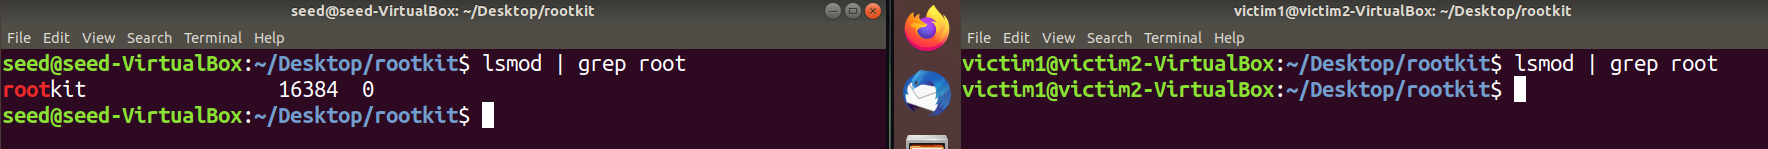
\includegraphics[width=\linewidth]{images/hide-lsmod.png}
    \caption{Hidden LKM from lsmod}
\end{figure}
\begin{figure}[H]
\centering
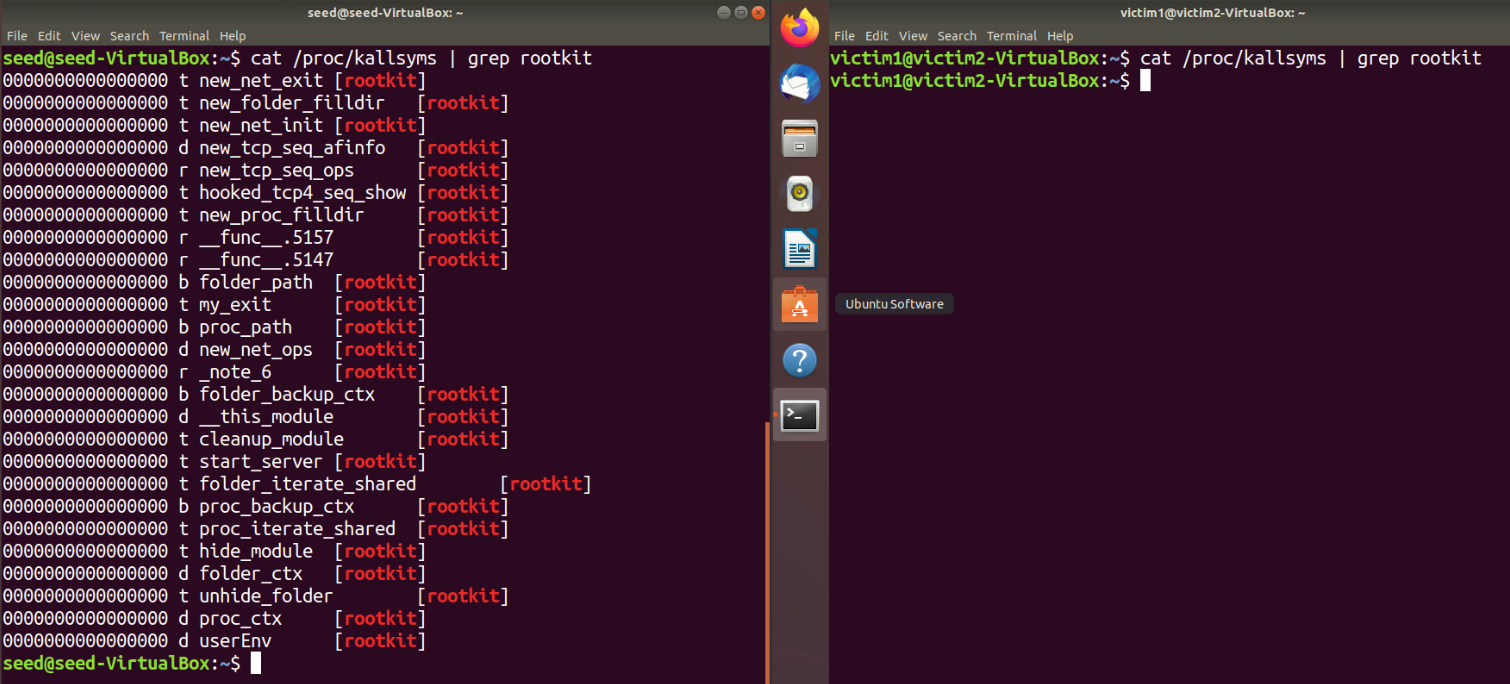
\includegraphics[width=\linewidth]{images/hide-kallsyms.png}
    \caption{Hidden LKM from /proc/kallsyms}
\end{figure}
\begin{figure}[H]
\centering
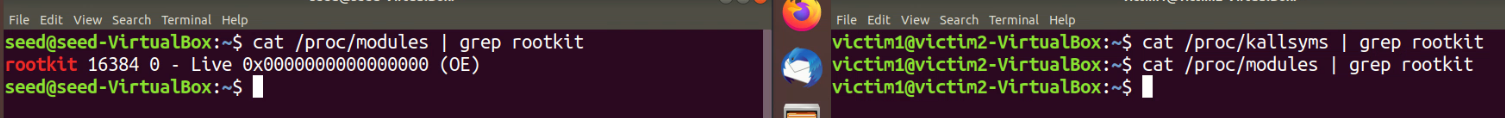
\includegraphics[width=\linewidth]{images/hide-proc-modules.png}
    \caption{Hidden LKM from /proc/modules}
\end{figure}
\begin{figure}[H]
\centering
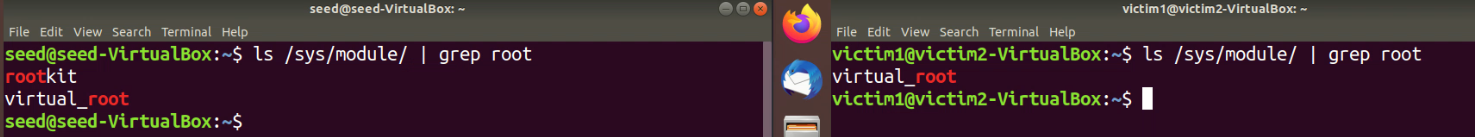
\includegraphics[width=\linewidth]{images/hide-sys-module.png}
    \caption{Hidden LKM from /sys/module}
\end{figure}
\begin{figure}[H]
\centering
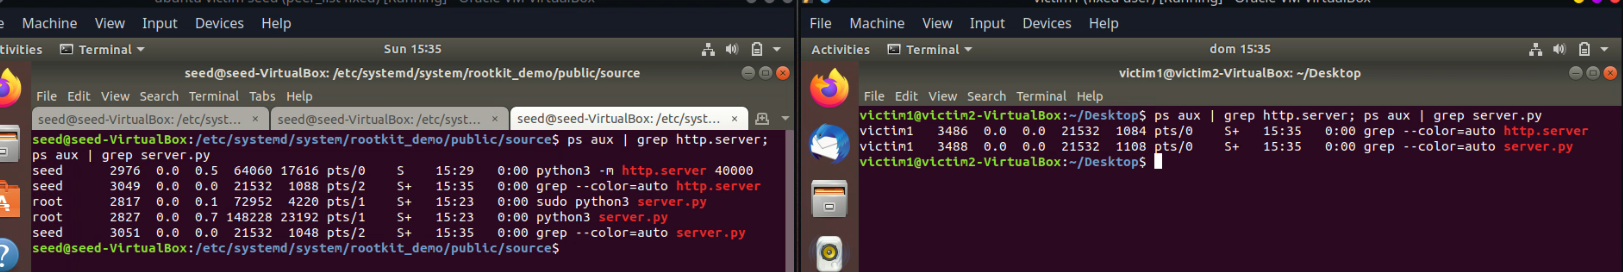
\includegraphics[width=\linewidth]{images/hide-ps.png}
    \caption{Hidden processes}
\end{figure}
\begin{figure}[H]
\centering
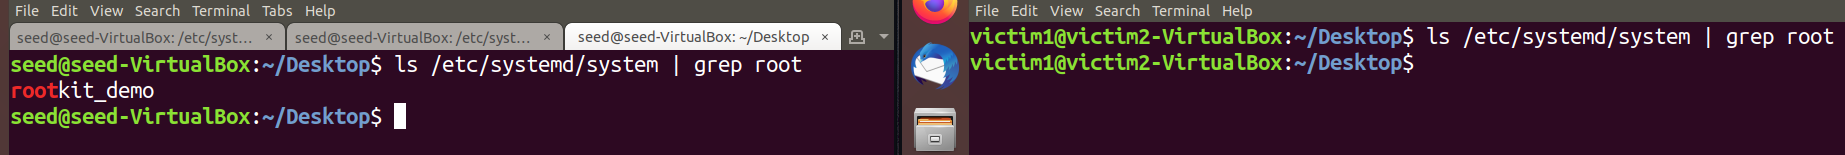
\includegraphics[width=\linewidth]{images/hide-folder.png}
    \caption{Hidden folders}
\end{figure}
\begin{figure}[H]
\centering
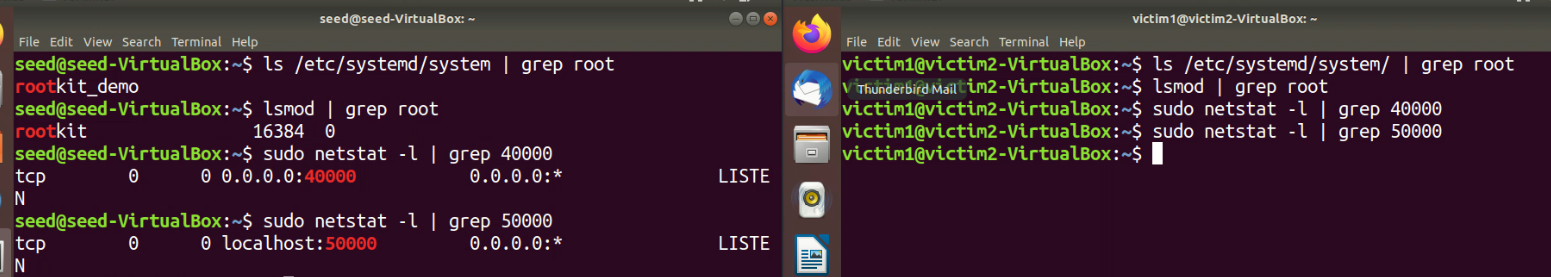
\includegraphics[width=\linewidth]{images/hide-lkm-netstat.png}
    \caption{Hidden netstat ports}
\end{figure}

Connect to a victim machine to obtain information is also possible. We just need to use the attacker's private key. In figure \ref{fig:victim-command}, we can see the output in the attacker shell on the right and the message debugged in a victim machine in the background. Furthermore, we can use anonymizers to increase security when accessing machines. Making it difficult to trace us back. We just need to specify the number of anonymizers when connecting to the victim machine.
\\
\begin{figure}[H]
\centering
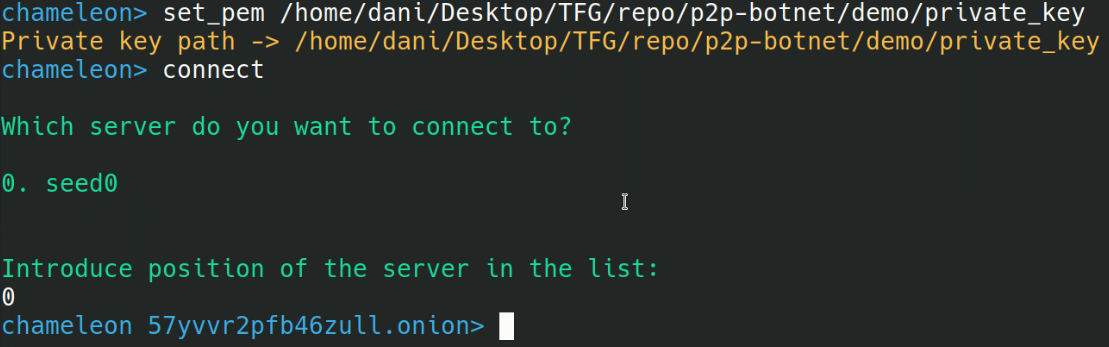
\includegraphics[width=\linewidth]{images/connect-to-victim.png}
    \caption{Establish connection to a victim machine}
\end{figure}
\begin{figure}[H]
\centering
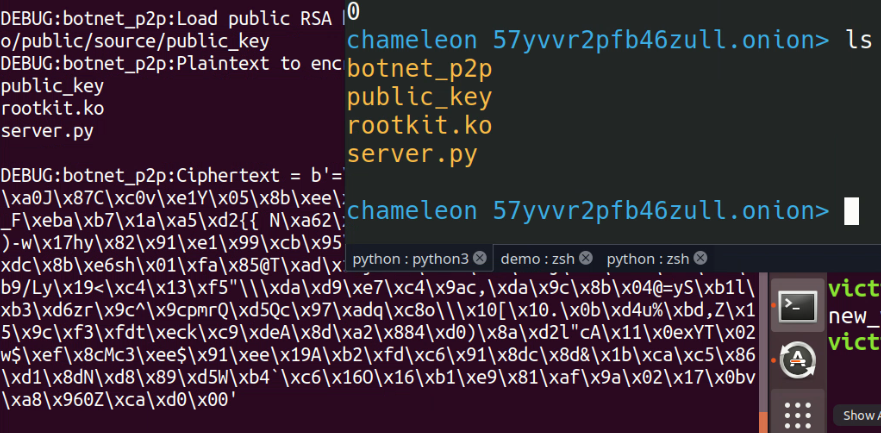
\includegraphics[width=\linewidth]{images/ls-victim.png}
    \caption{Executing an ls command on the victim machine}
    \label{fig:victim-command}
\end{figure}
\begin{figure}[H]
\centering
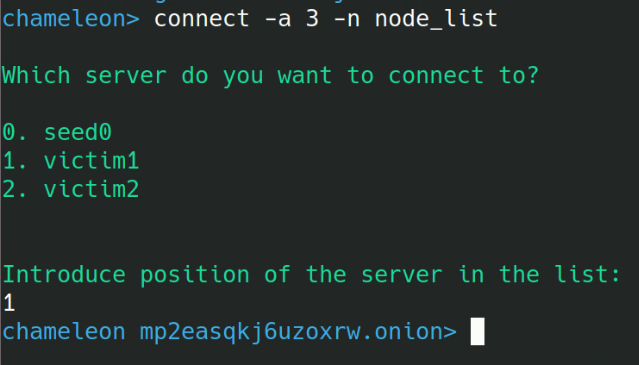
\includegraphics[width=\linewidth]{images/anonymizers-number.png}
    \caption{Connect to a victim through anonymizers}
    \label{fig:victim-command}
\end{figure}

Finally, we can update a file with a simple command given that at least one infected node has the updated file. In the message sent by the attacker, we need to include the hash of the file to update. This way, each victim knows whether it already has the updated file or not and can act accordingly. An important detail is that due to the implementation, we need the updated file in two computers: the master computer and a victim computer. We need it in the master's computer to calculate the hash of the file easily and in the victim machine so that the peers know from where to download it. With that configuration, we can update the file in the whole network.

\begin{figure}[h]
\centering
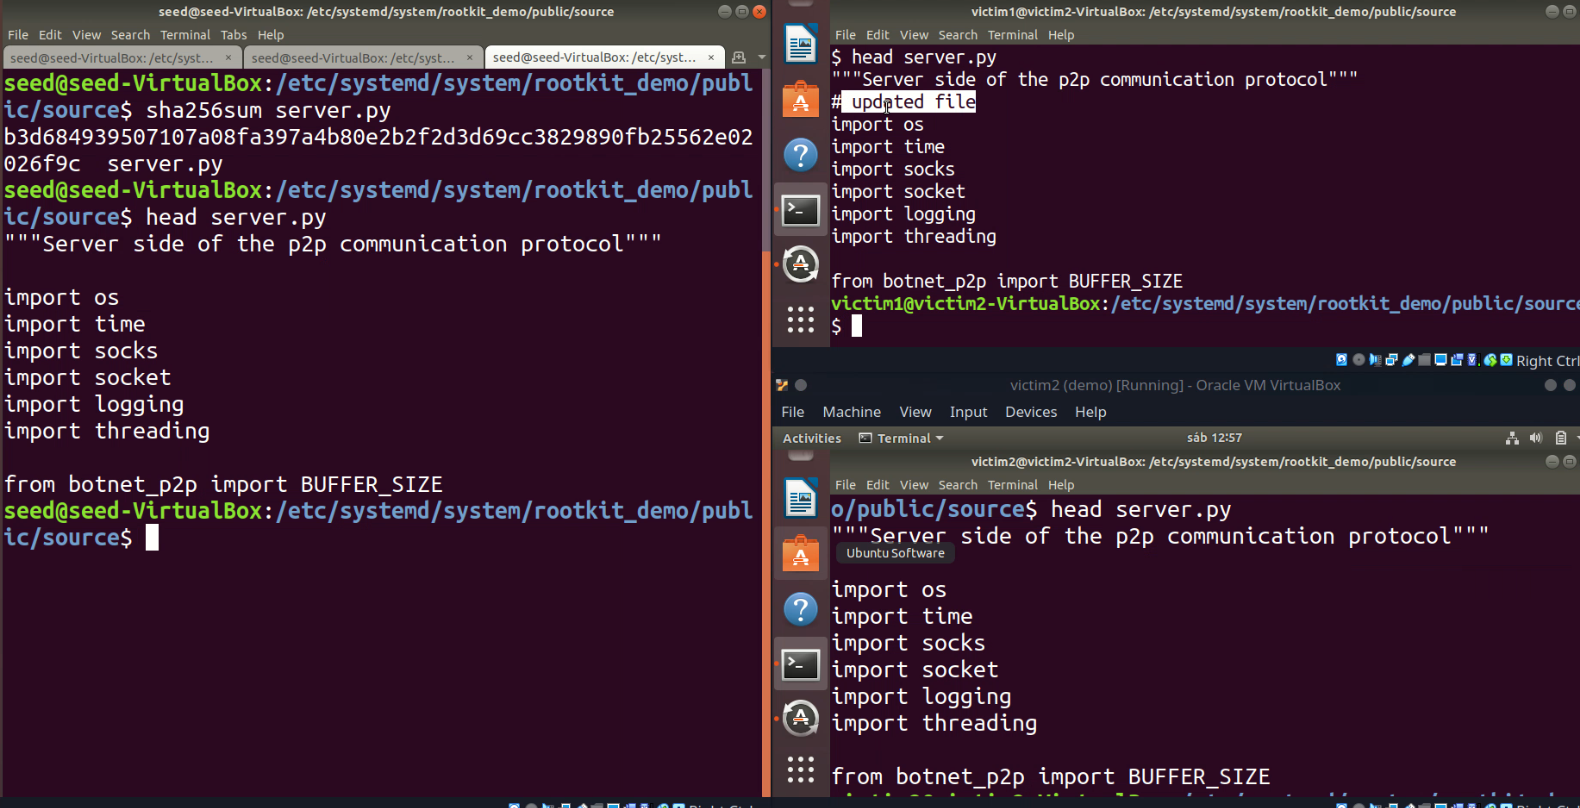
\includegraphics[width=\linewidth]{images/victim1-update.png}
    \caption{Victim1 holding the file to update in the other victims before executing the update command}
    \label{fig:victim-command}
\end{figure}
\begin{figure}[H]
\centering
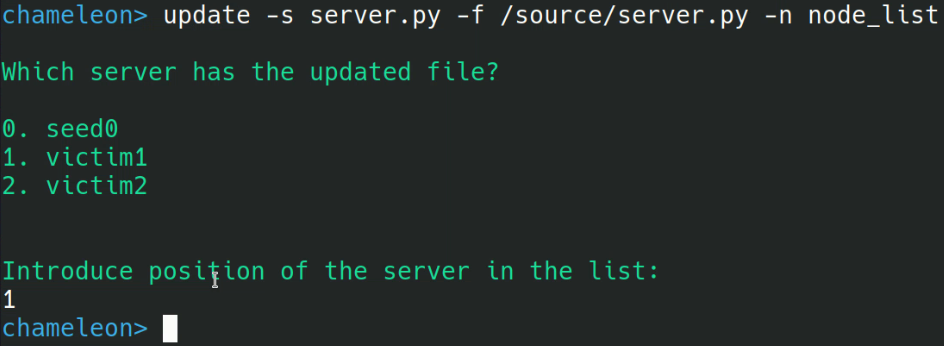
\includegraphics[width=\linewidth]{images/update-command.png}
    \caption{Update command example}
    \label{fig:victim-command}
\end{figure}
\begin{figure}[h]
\centering
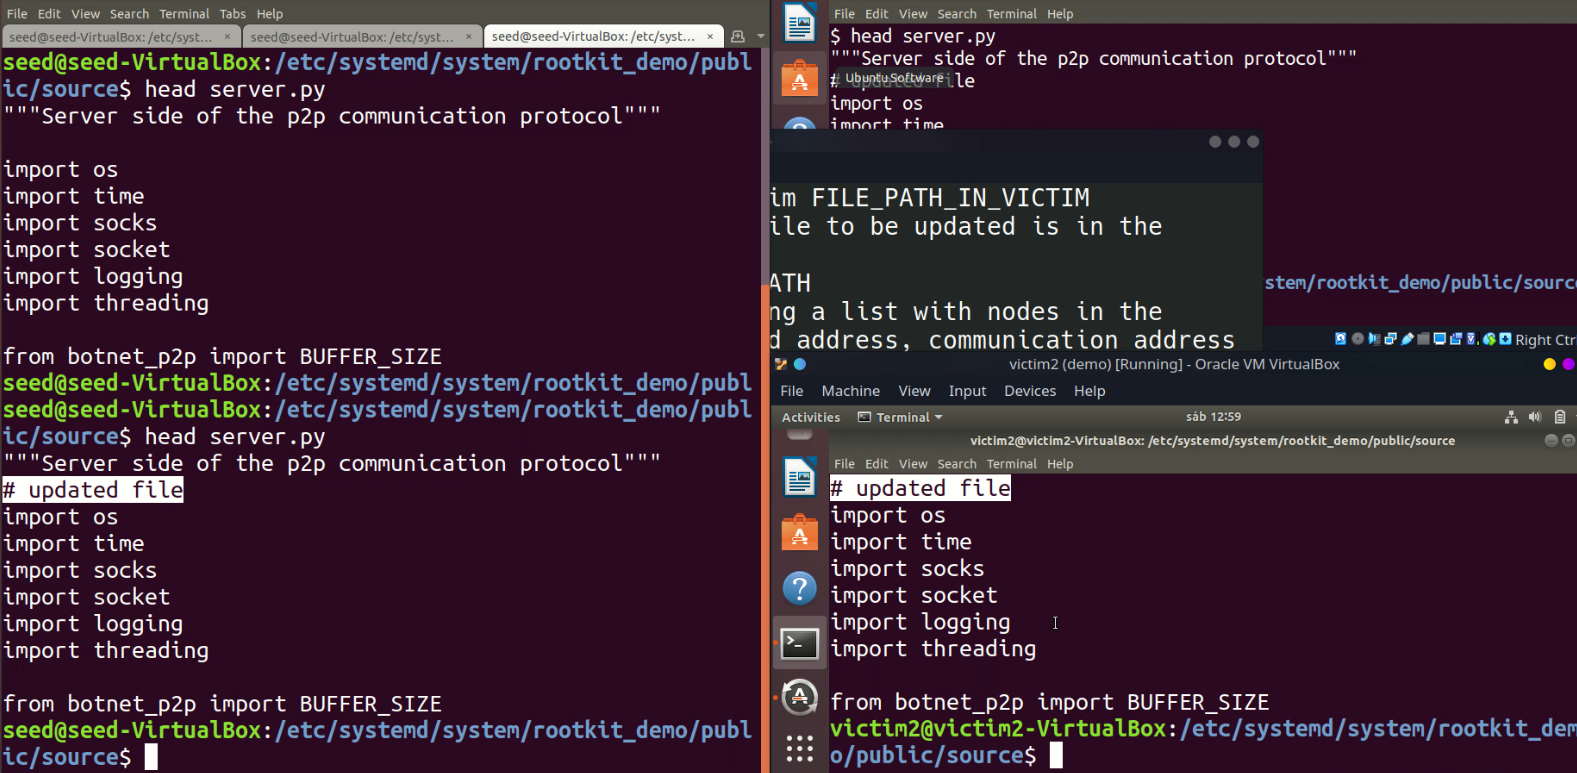
\includegraphics[width=\linewidth]{images/updated-files.png}
    \caption{Peer files updated after executing the update command}
    \label{fig:victim-command}
\end{figure}

\section{Future research}

The proposed botnet is far from perfect. It has some disadvantages that could be improved with further research.

The botnet heavily depends on the initial seeds to bootstrap the botnet and infect its first victims. Someone could DoS the seed machines and stop our botnet from growing. Eliminating this dependency would increase the botnet resiliency in its initial state. Research on P2P bootstrapping algorithms could help. Furthermore, using an Ethereum smart contract is also feasible \cite{blockchain-botnet} and could maybe remove our dependency on seed machines.

The infection vector is rather simple and general. We send an email with an attached malicious file and hope the user to download and open it. However, every user has different habits, skills, knowledge ..., and if we are targeting specific people, this is not our best move. To maximize the likelihood of the user being infected, the cybercriminal must make an investigation about the person and adjust the infection vector. That can be error-prone and subjective to the cybercriminal experience. Artificial Intelligence techniques could help us tailor the infection vector to each person.

Infecting machines may not always be what we want. Malware could end in honeypots \footnote{Machine or set of machines used as a decoy or trap to attract cybercriminals' attention. Used to avoid attacks and learn from them} or virtual machines set up by researchers. In both cases, they want to investigate how our malware and botnet works. We do not know if a machine is a trap or not. Artificial Intelligence techniques could help us avoid traps. Therefore, obtaining a stealthier botnet.

Our botnet uses Tor communication protocol and we are vulnerable to the attacks that Tor is vulnerable. Mixing various anonymizing networks could help us avoiding some attacks since we would jump between networks. Making it harder to follow our track.

We believe that these are some of the most interesting vulnerabilities to investigate how to improve them.

\section{Basic good practices}

Looking to our botnet, to infect machines, people must download and open the file with a vulnerable application, vim in this case. We cannot stress enough how important it is to keep applications and systems up to date. They are usually done for two things: new features or security updates. So installing them is important. Furthermore, you must always suspect anyone on the internet. Never download and execute files from sources that you cannot double-check they are the origin. If some of your friends send you an email with a file, text, or call him to make sure the emails come directly from him. Social Engineering is too powerful, do not overestimate its power.

From a technical point of view, encouraging people to make secure choices by default and researching about zero-days exploits can make the difference.

\clearpage
\chapter{Conclusion}

Botnets are systems used by cybercriminals for any kind of task, they will not disappear any time soon. We have shown how easy it is to hide the malware from the Linux kernel and steal the user information. People use computers to make their life easier, not to worry about privacy and security. Engineers must make systems and applications secure, even when users do not take the most secure options. Although it can be very difficult.


\bibliography{bibliography.bib}



\backmatter
\printindex





\end{document}


%NUMBER OF THE EXTERNAL PAGE EXCEPT IN THE FIRST PAGE OF EACH CAPITAL
\usepackage{fancyhdr}
\pagestyle{fancy}
\fancyfoot{}
\fancyfoot[RO]{\thepage}
\fancyfoot[LE]{\thepage}


%MULTIPLE INDEX
%In the preamble
\usepackage{multind}
\makeindex{authors}
%Introduction to form entries
\index{authors}{Einstein}
%Situation of the Index
\printindex{authors}{Author index}
%The \ usepakage {makeidx} \ makeindex \ printindex commands must be removed
%You need to exacute from the command line makeindex authors